%\documentclass[journal]{vgtc}                % final (journal style)
\documentclass[review,journal]{vgtc}         % review (journal style)
%\documentclass[widereview]{vgtc}             % wide-spaced review
%\documentclass[preprint,journal]{vgtc}       % preprint (journal style)

%% Uncomment one of the lines above depending on where your paper is
%% in the conference process. ``review'' and ``widereview'' are for review
%% submission, ``preprint'' is for pre-publication, and the final version
%% doesn't use a specific qualifier.

%% Please use one of the ``review'' options in combination with the
%% assigned online id (see below) ONLY if your paper uses a double blind
%% review process. Some conferences, like IEEE Vis and InfoVis, have NOT
%% in the past.

%% Please note that the use of figures other than the optional teaser is not permitted on the first page
%% of the journal version.  Figures should begin on the second page and be
%% in CMYK or Grey scale format, otherwise, colour shifting may occur
%% during the printing process.  Papers submitted with figures other than the optional teaser on the
%% first page will be refused. Also, the teaser figure should only have the
%% width of the abstract as the template enforces it.

%% These few lines make a distinction between latex and pdflatex calls and they
%% bring in essential packages for graphics and font handling.
%% Note that due to the \DeclareGraphicsExtensions{} call it is no longer necessary
%% to provide the the path and extension of a graphics file:
%% 
\includegraphics{diamondrule} is completely sufficient.
%%
\ifpdf%                                % if we use pdflatex
  \pdfoutput=1\relax                   % create PDFs from pdfLaTeX
  \pdfcompresslevel=9                  % PDF Compression
  \pdfoptionpdfminorversion=7          % create PDF 1.7
  \ExecuteOptions{pdftex}
  \usepackage{graphicx}                % allow us to embed graphics
                                % files
  \DeclareGraphicsExtensions{.pdf,.png,.jpg,.jpeg} % for pdflatex we expect .pdf, .png, or .jpg files
\else%                                 % else we use pure latex
  \ExecuteOptions{dvips}
  \usepackage{graphicx}                % allow us to embed graphics files
  \DeclareGraphicsExtensions{.eps}     % for pure latex we expect eps files
\fi%

%% it is recomended to use ``\autoref{sec:bla}'' instead of ``Fig.~\ref{sec:bla}''
\graphicspath{{figures/}{pictures/}{images/}{./}{img/}} % where to search for the images

\usepackage{microtype}                 % use micro-typography (slightly more compact, better to read)
\PassOptionsToPackage{warn}{textcomp}  % to address font issues with \textrightarrow
\usepackage{textcomp}                  % use better special symbols
\usepackage{mathptmx}                  % use matching math font
\usepackage{times}                     % we use Times as the main font
\renewcommand*\ttdefault{txtt}         % a nicer typewriter font
\usepackage{cite}                      % needed to automatically sort the references
\usepackage{tabu}                      % only used for the table example
\usepackage{booktabs}                  % only used for the table example
\usepackage{color}
%\usepackage{algorithmic}
% \usepackage[]{algorithm2e}
%\usepackage[algo2e]{algorithm2e} 
\usepackage{amsmath}
\usepackage{amsfonts}
\usepackage{algorithm,algpseudocode}
%\usepackage{algpseudocode}
%\usepackage{algorithm}
\usepackage[dvipsnames]{xcolor}
\usepackage{xspace}
\algnewcommand{\Inputs}[1]{%
  \State \textbf{Inputs:}
  \Statex \hspace*{\algorithmicindent}\parbox[t]{.9\linewidth}{\raggedright #1}
}
\algnewcommand{\Output}[1]{%
  \State \textbf{Output:}
  \Statex \hspace*{\algorithmicindent}\parbox[t]{.9\linewidth}{\raggedright #1}
}
\algnewcommand{\Initialize}[1]{%
  \State \textbf{Initialize:}
  \Statex \hspace*{\algorithmicindent}\parbox[t]{.8\linewidth}{\raggedright #1}
}
%%\newcommand{\norm}[1]{\left\lVert#1\right\rVert}
%% We encourage the use of mathptmx for consistent usage of times font
%% throughout the proceedings. However, if you encounter conflicts
%% with other math-related packages, you may want to disable it.

%% In preprint mode you may define your own headline.
%\preprinttext{To appear in IEEE Transactions on Visualization and Computer Graphics.}

%% If you are submitting a paper to a conference for review with a double
%% blind reviewing process, please replace the value ``0'' below with your
%% OnlineID. Otherwise, you may safely leave it at ``0''.
\onlineid{1207}

%% declare the category of your paper, only shown in review mode
\vgtccategory{Research}
%% please declare the paper type of your paper to help reviewers, only shown in review mode
%% choices:
%% * algorithm/technique
%% * application/design study
%% * evaluation
%% * system
%% * theory/model
\vgtcpapertype{Evaluation}

%% Paper title.
\title{A Study of the Tradeoff between Reducing Precision and Reducing Resolution for Data Analysis and Visualization}

%% This is how authors are specified in the journal style

%% indicate IEEE Member or Student Member in form indicated below
\author{Duong Hoang, Pavol Klacansky, Harsh Bhatia, Peer-Timo Bremer, Peter Lindstrom, Valerio Pascucci}
\authorfooter{
%% insert punctuation at end of each item
\item
 Hoang, Klacansky, and Pascucci are with the SCI Institute at the University of Utah, USA. E-mail: \{duong, klacansky, pascucci\}@sci.utah.edu
\item
 Bhatia, Bremer, and Lindstrom are with Lawrence Livemore National Laboratory, USA. E-mail: \{hbhatia, bremer5, pl\}@llnl.gov
}

%other entries to be set up for journal
\shortauthortitle{Hoang \MakeLowercase{\textit{et al.}}: Studying the Tradeoff between Reducing Precision and Reducing Resolution for Data Analysis and Visualization}

%% Abstract section.
\abstract{There currently exist two dominant strategies to reduce data sizes in analysis and
  visualization: reducing the {\it precision} of the data, e.g., through compression, or reducing
  its {\it  resolution}, e.g., by subsampling. Both have advantages and disadvantages and both face
  fundamental limits at which the reduced information ceases to be useful. The paper explores the
  additional gains that could be achieved by combining both strategies. In particular, we present a
  common framework that allows us to study the trade-off in reducing precision and/or resolution in
  a principled manner. We represent data reduction schemes as a progressive stream of bits, and
  study how various bit orderings such as by resolution, by precision, etc. impact the resulting
  approximation error across a wide range of test data and analysis tasks. Furthermore, we compute
  streams optimized for different tasks, to serve as lower bounds on the achievable error.
  Scientific data management systems can use the results presented in this paper as guidance on how
  to store and stream data to make efficient use of the limited storage and bandwidth in practice.


% Performing scientific analysis on large data commonly found nowadays is an onerous task
% due to the prohibitive cost of data transfer. Currently, this issue is alleviated by working with
% reduced-resolution or reduced-precision data.
% \peter{Mention progressive access here?}
% This paper brings together techniques that reduce data
% in resolution, precision, or both, into a common framework in which they can be studied and
% compared. The error patterns of these techniques are compared in terms of fundamental error metrics on function values (e.g., L2 norm),
% first and second derivatives, histograms, and isocontours. We also compute and study
% metric-dependent streams
% \peter{streams optimized for different metrics?}
% that serve as empirical bounds on the limit to which
% reduction can happen, given an error tolerance for the analysis task at hand. Finally, based on the
% observed characteristics of those streams, we propose practical heuristics to minimize the amount of data
% needed to perform a given analysis task. The insights and heuristics presented here can be
% leveraged to implement data-optimal\pavol{"optimal" or other word?}
% \peter{what does data-optimal representations of data mean?}
% representations and querying systems
% \peter{query systems?  I.e., a noun, not a verb?}
% to facilitate interactive
% exploration as well as cursory analysis of enormous data.%
% \peter{The abstract does not make it clear what it is we're optimizing,
% i.e. ordering of bits.}
} % end of abstract

%% Keywords that describe your work. Will show as 'Index Terms' in journal
%% please capitalize first letter and insert punctuation after last keyword
% \keywords{Radiosity, global illumination, constant time}

%% ACM Computing Classification System (CCS). 
%% See <http://www.acm.org/class/1998/> for details.
%% The ``\CCScat'' command takes four arguments.

\CCScatlist{ % not used in journal version
 \CCScat{K.6.1}{Management of Computing and Information Systems}%
{Project and People Management}{Life Cycle};
 \CCScat{K.7.m}{The Computing Profession}{Miscellaneous}{Ethics}
}

%% Uncomment below to include a teaser figure.
\teaser{
  \centering
  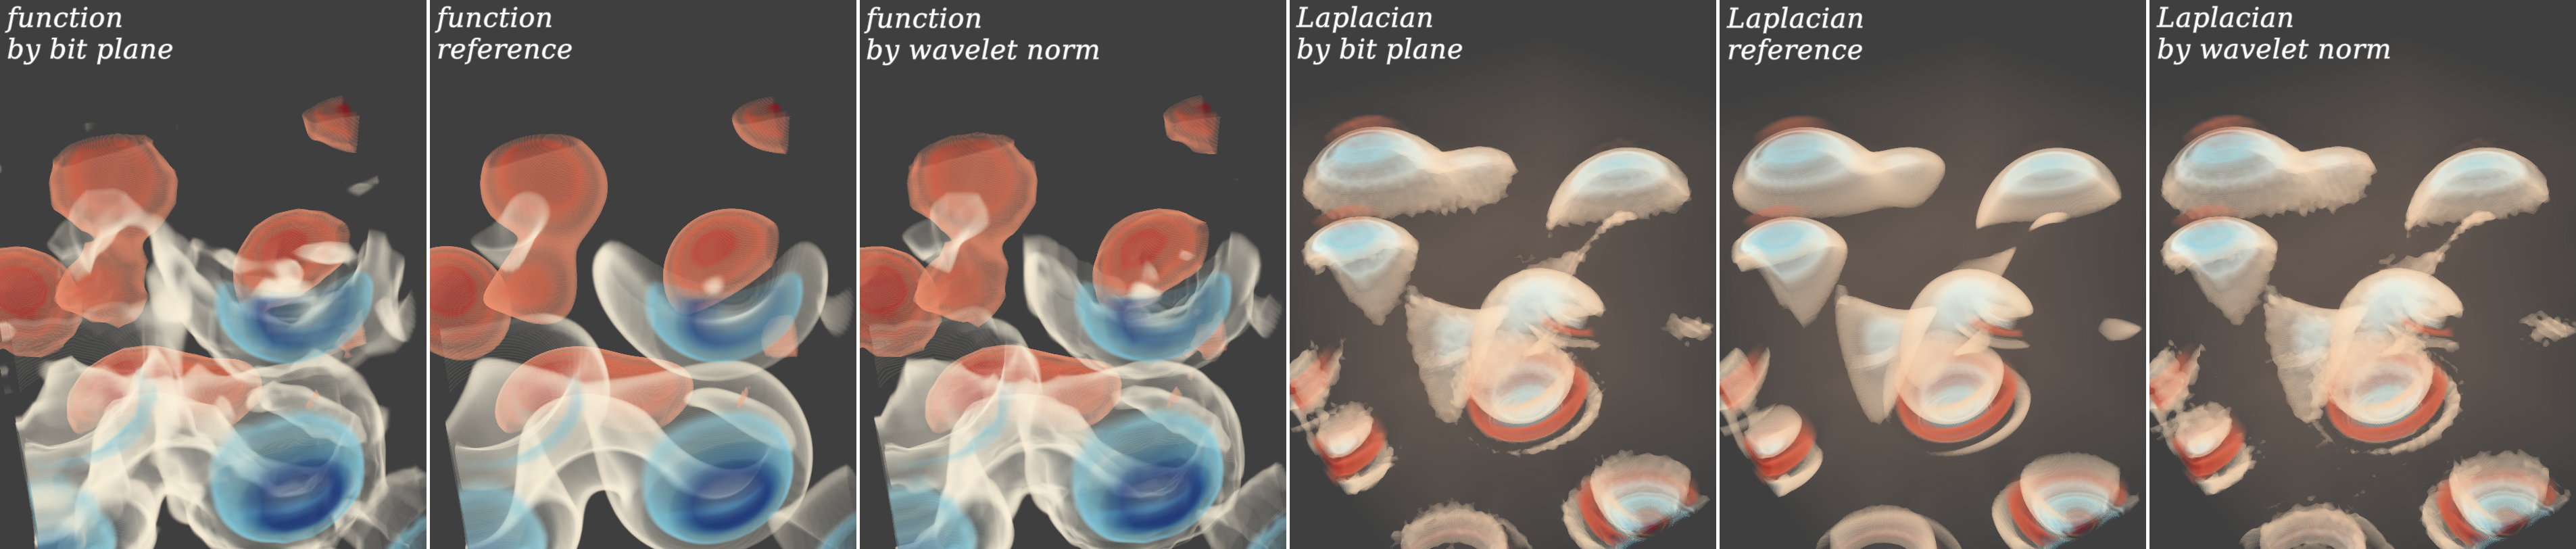
\includegraphics[width=0.99\linewidth]{cats}
  % \subcaptionbox{By level}{
  % {\includegraphics[width=0.15\linewidth]{teaser_rmse_level}}}
  % \subcaptionbox{By bit plane}{
  % {\includegraphics[width=0.15\linewidth]{teaser_rmse_bit_plane}}}
  % \subcaptionbox{By wavelet norm}{
  % {\includegraphics[width=0.15\linewidth]{teaser_rmse_wavelet_norm}}}
  % \subcaptionbox{Signature}{
  % {\includegraphics[width=0.15\linewidth]{teaser_rmse_signature}}}
  % \subcaptionbox{Groundtruth}{
  % {\includegraphics[width=0.15\linewidth]{teaser_rmse_groundtruth}}}
  % \\
  % \subcaptionbox{By level}{
  % {\includegraphics[width=0.15\linewidth]{teaser_laplacian_level}}}
  % \subcaptionbox{By bit plane}{
  % {\includegraphics[width=0.15\linewidth]{teaser_laplacian_bit_plane}}}
  % \subcaptionbox{By wavelet norm}{
  % {\includegraphics[width=0.15\linewidth]{teaser_laplacian_wavelet_norm}}}
  % \subcaptionbox{By signature}{
  % {\includegraphics[width=0.15\linewidth]{teaser_laplacian_signature}}}
  % \subcaptionbox{Groundtruth}{
  % {\includegraphics[width=0.15\linewidth]{teaser_laplacian_groundtruth}}}
  \caption{Renderings of the \emph{diffusivity} field at 0.1 bits per sample (bps), and its Laplacian field, at 0.6 bps, using two of the bit streams studied in the paper. Compared to the \emph{by bit plane} stream, \emph{by wavelet norm} produces a better reconstruction of the original function (left, see white features), but a worse reconstruction of the Laplacian field (right).}
  \label{fig:teaser}
}

%% Uncomment below to disable the manuscript note
%\renewcommand{\manuscriptnotetxt}{}


\newcommand{\norm}[1]{\left\lVert#1\right\rVert}
\newcommand{\notetext}[1]{%
  \raggedright\tiny\sffamily\bfseries{#1}%
}
\newcommand{\note}[1]{%
  \ifinner%
    \smash{%
      \raggedright%
      \hspace*{\textwidth}%
      \hspace*{\marginparsep}%
      \parbox[t]{\marginparwidth}{\notetext{#1}}%
    }%
    \\[-0.5\bs]%
  \else%
    \marginpar{\notetext{#1}}%
  \fi%
}
\providecommand{\etal}{et al.\@\xspace}

\usepackage[normalem]{ulem}
\newcommand{\pavol}[1]{{\textcolor{cyan}{(Pavol: #1)}}}
\newcommand{\hb}[1]{{\textcolor{blue}{(HB: #1)}}}
\newcommand{\hbadd}[1]{{\textcolor{blue}{#1}}}
\newcommand{\hbdel}[1]{{\textcolor{red}{Delete: #1}}} % was failing on my machine
%\newcommand{\hbdel}[1]{{\textcolor{red}{}}}
\newcommand{\todo}[1]{{\textcolor{red}{#1}}}
%\newcommand{\duong}[1]{{\textcolor{purple}{(Duong: #1)}}}
\newcommand{\duong}[1]{{\textcolor{purple}{}}} % this disable comments
\newcommand{\peter}[1]{{\textcolor{green}{(PL: #1)}}} % this disable comments
\newcommand{\ptb}[1]{{\textcolor{violet}{(PTB: #1)}}} % this disable comments

% prevent hyphenation
\usepackage[none]{hyphenat}
\sloppy

% ignore figures for fast compilation
% \usepackage[allfiguresdraft]{draftfigure}

\usepackage[mathcal]{euscript}

\newcommand {\mm}[1] {\ifmmode{#1}\else{\mbox{\(#1\)}}\fi}

\newcommand{\Lspace}{{\mathbb L}}
\newcommand{\strm}	{\mm{\mathcal{S}}\xspace}
\newcommand{\sgn}	{\mm{\Lambda}\xspace}
\newcommand{\sopt}  {\mm{\strm_{\text{opt}}}\xspace}
\newcommand{\slvl}  {\mm{\strm_{\text{lvl}}}\xspace}
\newcommand{\sbit}  {\mm{\strm_{\text{bit}}}\xspace}
\newcommand{\swav}  {\mm{\strm_{\text{wav}}}\xspace}
\newcommand{\smag}  {\mm{\strm_{\text{mag}}}\xspace}
\newcommand{\ssig}  {\mm{\strm_{\text{sig}}}\xspace}
\newcommand{\stkop}  {\mm{\strm_{\text{[task]-opt}}}\xspace}
\newcommand{\stksg}  {\mm{\strm_{\text{[task]-sig}}}\xspace}
\newcommand{\srop}  {\mm{\strm_{\text{rmse-opt}}}\xspace}
\newcommand{\srsg}  {\mm{\strm_{\text{rmse-sig}}}\xspace}
\newcommand{\sgop}  {\mm{\strm_{\text{grad-opt}}}\xspace}
\newcommand{\sgsg}  {\mm{\strm_{\text{grad-sig}}}\xspace}
\newcommand{\slop}  {\mm{\strm_{\text{lap-opt}}}\xspace}
\newcommand{\slsg}  {\mm{\strm_{\text{lap-sig}}}\xspace}
\newcommand{\shop}  {\mm{\strm_{\text{hist-opt}}}\xspace}
\newcommand{\shsg}  {\mm{\strm_{\text{hist-sig}}}\xspace}
\newcommand{\siop}  {\mm{\strm_{\text{iso-opt}}}\xspace}
\newcommand{\sisg}  {\mm{\strm_{\text{iso-sig}}}\xspace}

% stream weights
%\newcommand{\wlvl}  {\mm{w_{\text{lvl}}}\xspace}
%\newcommand{\wbit}  {\mm{w_{\text{bit}}}\xspace}
%\newcommand{\wwav}  {\mm{\mathcal{W}_{\text{wav}}}\xspace}
\newcommand{\wwav}  {\mm{w_{\text{wav}}}\xspace}
\newcommand{\wmag}  {\mm{w_{\text{mag}}}\xspace}

% wavelet coeff and basis
\newcommand{\wcof}  {\mm{w}\xspace}
\newcommand{\wbas}  {\mm{\psi}\xspace}
\newcommand{\wsca}  {\mm{\phi}\xspace}

\newcommand{\err}   {\mm{\varepsilon}\xspace}
\newcommand{\x}     {\mm{\mathbf{x}}\xspace}

\newcommand{\para}[1]{\vspace{0.5em}\noindent{\textbf{#1}}}%\hspace{0.04em}}

\usepackage{pifont}% http://ctan.org/pkg/pifont
\newcommand{\cmark}{{\color{ForestGreen}{\ding{51}}}}%
\newcommand{\xmark}{{\color{red}{\ding{55}}}}%

%% Copyright space is enabled by default as required by guidelines.
%% It is disabled by the 'review' option or via the following command:
% \nocopyrightspace

\vgtcinsertpkg
%\usepackage{subcaption}
\usepackage[labelfont=sf]{subcaption}
\captionsetup{labelfont=sf,font=scriptsize,textfont=sf}
\usepackage{cleveref}
\Crefformat{figure}{#2Fig.~#1#3}

%%%%%%%%%%%%%%%%%%%%%%%%%%%%%%%%%%%%%%%%%%%%%%%%%%%%%%%%%%%%%%%%
%%%%%%%%%%%%%%%%%%%%%% START OF THE PAPER %%%%%%%%%%%%%%%%%%%%%%
%%%%%%%%%%%%%%%%%%%%%%%%%%%%%%%%%%%%%%%%%%%%%%%%%%%%%%%%%%%%%%%%%

\begin{document}

%% The ``\maketitle'' command must be the first command after the
%% ``\begin{document}'' command. It prepares and prints the title block.

%% the only exception to this rule is the \firstsection command

\firstsection{Introduction}
\maketitle

As the gap between the available compute power and the cost of data movement increases, data
transfer, whether from cache, main memory, or from disk, becomes a major bottleneck in many
workflows. However, it has been shown that not every bit of data is always necessary to answer
scientific questions with required accuracy. In particular, for techniques at the end of scientific
workflows, such as visualization and data analysis, lower fidelity representations of the data often
provide adequate approximations~\cite{woodring2011,covra2012,compression_sim2013}, and even during
simulation some loss in precision is often
acceptable~\cite{compression_sim2013,doi:10.1177/1094342018762036}. As a result, several different
techniques have been proposed to reduce the size of data. 

Broadly, these techniques can be classified into (i) reducing the data resolution, e.g., the number
of data points stored, and (ii) reducing the precision of each data point. Examples of the former
kind of approaches are subsampling~\cite{idx2001}, adaptive mesh refinement~\cite{amr1989}, octrees
and other tree structures~\cite{hierarchical1984}, and wavelets~\cite{woodring2011}, and those of
the latter are various forms of
compression~\cite{fpzip,isabela,zfp2014,sz,vq1992,compression_domain2003,sqe}. Traditionally,
multiresolution structures have been used to accelerate dynamic queries, e.g., in
rendering~\cite{multires_octree1999}, since discarding data points based on the viewpoint or data
complexity can result in significant speed-up. Compression based on quantization, on the other hand,
is more common when storing data, where in the absence of other information, treating each sample as
equally important is the null hypothesis. However, in many situations, a combination of both
resolution and precision reduction could be appropriate. For example, high spatial resolution may be
needed to resolve the topology of an isosurface, yet the corresponding data samples may be usable at
less than full precision to adequately approximate the geometry. Conversely, accumulating accurate
statistics may require high-precision values, yet a lower resolution subset of data points may be
sufficient for the task. 

In general, different levels of adaptivity in combinations of resolution and precision may be
suitable for different types of analysis and visualization tasks, and for many, these requirements
will be data dependent. Consequently, a globally optimal data organization may not exist. Instead,
we consider a progressive setting in which some initial data is loaded and processed, and new data
is requested selectively based on the requirement of the current task as well as the characteristics
of the data already loaded. The result is a stream of bits ordered such that the error is minimized,
considering the task at hand. However, although intuitively there are almost certainly advantages in
considering both resolution and precision in the ordering, it is unclear how much the error could be
reduced for a given data budget or how little data could be used to achieve the same error.
Furthermore, optimal data-dependent orderings may be especially impractical since they assume
perfect knowledge of the data. It is therefore important to understand which of these potential
gains are realizable. This paper aims to answer these important questions about the suitable bit
orderings through extensive, empirical experiments. In particular, this paper presents:

\begin{itemize}\dense
%
\item a framework that allows systematic studies of the resolution-versus-precision tradeoffs for
common data analysis and visualization tasks. The core idea is to represent various data reduction
techniques as bit streams that improve data quality in either resolution or precision in each step
(\Cref{sec:terminologies}). We can thus compare these techniques fairly, by comparing the
corresponding data streams.
%  
\item empirical evidence that jointly optimizing resolution and precision can provide significant
improvements on the results of analysis tasks over adjusting either independently. 
We present a diverse collection of data sets and data analysis tasks, and also show how
different types of data analysis might require substantially different data streams for optimal
results.
%
\item a greedy approach that gives estimations for lower bounds of error for various analysis tasks.
In addition, we also identify practical streams that closely approximate these bounds for each task
(\Cref{sec:rmse-optimized}, \Cref{sec:derivatives}, \Cref{sec:histogram}, and
\Cref{sec:isocontour}), using a novel concept called \emph{stream signature}
(\Cref{sec:stream-signature}), which is a small matrix that captures the essence of how a bit stream
navigates the precision-versus-resolution space.
\end{itemize}


%%% Local Variables:
%%% mode: latex
%%% TeX-master: "template"
%%% End:

\section{Related work}

\para{Tree-based multiresolution hierarchies.}
Techniques that reduce data in resolution typically build a tree-shape hierarchy over the data. A
very common scheme to generate such a hierarchy is to construct low-resolution copies of the data
from higher resolution ones through filtering or subsampling. Examples include Gaussian and
Laplacian pyramids~\cite{laplacian-pyramid},
mipmaps~\cite{multires_octree1999,interactive-exploration-ct-scans}. Often, the data is stored in
blocks on each resolution level. To save bandwidth, low-resolution blocks can be streamed during
rendering, if the points being queried project to less than a pixel on screen. However, these
methods increase storage requirements and potentially expensive pre-processing, making them
unsuitable for very large data.

Recent multi-resolution techniques save storage by adapting to the data in such a way that different
regions of the data are stored in different resolutions and depending on how ``homogeneous'' is the region.
Fast-varying regions are stored at higher resolution. A very popular approach is sparse voxel
octrees (SVO), pioneered by Crassin \etal~\cite{gigavoxels} and Gobbetti \etal~\cite{Gobbetti2008},
and variations of which are found in~\cite{Fogal-2013-RayGuided,visualization-driven}. Sparsity
comes from the fact that smooth-varying regions are stored at coarser octree levels, which
significantly reduces storage. During rendering, blocks of samples are streamed from an appropriate
resolution, determined by how far the queried samples are from the eye/camera. Beyer
\etal~\cite{large‐scale-volume} give a comprehensive overview of state-of-the-art GPU-based
out-of-core ray-casting techniques.

Beside octrees, other trees such as B+ tree~\cite{vdb2013} and
kd-tree~\cite{fogal-kdtree,in-situ-sampling-particle} can also be used to build a sparse hierarchy.
Alternatively, space-filling curves such as the hierarhical Z curve~\cite{idx2001} or the Hillbert
curve~\cite{mloc} can be used to reorder data samples to form a hierarchy without any filtering
steps or redundant samples, as low-resolution levels are constructed via subsampling. Unfortunately,
subsampling can introduce aliasing.

%\paragraph{\textbf{Transform-based multiresolution hierarchies}}
\para{Transform-based multiresolution hierarchies.}
Other multiresolution approaches reduce data by transform-based compression. For example,
COVRA~\cite{covra2012} constructs an octree of bricks, each of which is further subdivided \pavol{into?} blocks.
Compression is done by learning a sparse representation for the blocks in terms of prototype (basis)
blocks. Similarly, Fout\etal~\cite{hw_dvr2007} transform each block in the volume using the KLT
transform, which produces several classes of partitions (each can be thought of as one resolution
level). They compress the transform coefficients using vector quantization~\cite{vq1992} by
constructing one codebook for each paritition class. Schneider~\etal~\cite{compression_domain2003}
also use vector quantization on transform coefficients, but with a simple Haar-like transform that
separates each block of $2^3$ voxels into one average and seven difference coefficients.

Analogous to the KLT transform in 2D, the Tucker decomposition~\cite{tensor_dvr2015} in
$n$-dimensional space decomposes the input data (stored as a tensor) into $n$ matrices of basis
vectors and one core tensor. Reduction in storage and in transmission bandwidth comes from the fact
that the basis matrices can be downsampled (resulting in a lower resolution representation) and the
core tensor can be rank-truncated (resulting in coarse-scale representations of
features)~\cite{tamresh,tucker-thresholding,multiscale-tensor}. Furthermore, elements in the basis
matrices and the core tensor can be thresholded~\cite{tucker-thresholding} or
quantized~\cite{tamresh,multiscale-tensor}. Tensor decomposition can work for higher dimensional
data and can achieve very high compression ratios. However, the transform step is costly due to it
being data-dependent.

%\paragraph{\textbf{Wavelets}}
\para{Wavelets.}
Transforms that use fixed bases avoid such high computation cost at the expense of slightly less
effective compression. Perhaps the most popular transform that uses a fixed basis is the (discrete)
wavelet transform (DWT). The DWT constructs a hierarchy of resolution levels via low and high
bandpass filters. The transform is recursively applied to the lower resolution band, resulting in a
hierarchy of ``details'' at varying resolution. One benefit of wavelets over redundant
representations such as Laplacian pyramids is that the wavelet transform is merely a change of basis
that like reordering techniques does not increase the data size. Another benefit over adaptive
refinement meshes and other tree-like techniques is that the wavelet basis functions are defined
everywhere in space, requiring no special interpolation rules when given some arbitrary subset of
wavelet coefficients and basis functions. One disadvantage of the wavelet transform is the random
access cost, which is not constant time. However, there has been work to develop acceleration
structures to speed up local queries~\cite{weiss}.

Beside offering a multiresolution decomposition, enabling data streaming with level-of-detail
support, wavelets also offer ample opportunities for compression. As the magnitude of wavelet
coefficients decays rapidly for a typical volume [CITE], they are especially amenable to thresholding
or entropy compression. In the context of storing and visualizing scientific data, wavelets (with
compression) are used in a wide variety of
systems~(\cite{multires_toolkit2003,vapor2007,woodring2011}) and applications (volume rendering
with
level-of-detail~\cite{wavelet-compression-interactive-vis,multires-framework,rapid-compression-volume,interactive-rendering-large-volume,multires-volume-rendering},
turbulence visualization~\cite{treib}, particle visualization~\cite{sph-octree}).

Most wavelet-based techniques employ tiling of wavelet coefficients in individual subands to
facilitate random access and spatial adaptivity in resolution. For example, the VAPOR
toolkit~\cite{vapor2007} incorporates a multiresolution file format based on a wavelets to allow
data analysis on commodity hardware by storing individual tiles in separate files to allow loading
of the region of interest. However, like most multiresolution work, only the resolution control is
leveraged. The precision axis, which can potentially further reduce data transfer, is left
unexplored.

%\paragraph{\textbf{Wavelet coders}}
\para{Wavelet coders.}
Most work that explores the precision axis comes from state-of-the-art coders for wavelet
coefficients in image compression. Wavelet coefficients in corresponding regions across subbands can
be thought of as belonging to a ``tree'', with the root being a single coefficient at the lowest
subband. Thee emmbedded zerotrees (EZW) coder exploits the property that in such trees, ``parent''
coefficients are often larger in magnitude than ``child'' coefficients. It locates trees of wavelet
coefficients that are insignificant with regard to (i.e., less than in magnitude) a threshold. Such
a tree is encoded with one single symbol, resulting in significant compression. The threshold is
typically set at each bit plane, starting from the most significant one. In this way, the data can
be progressively refined in precision during decompression. The SPIHT coder~\cite{spiht1996}
improves on EZW by locating more general types of zero trees~\cite{quantifying-coding-performance}.
SPECK~\cite{speck2004} extends SPIHT to exploit also spatial correlations among nearby coefficients
on the same subband.

%\paragraph{\textbf{Floating-point compression}}
\para{Floating-point compression.}
\newcommand{\zfp}{\textsc{zfp}\xspace}
The \zfp compression scheme~\cite{zfp2014} also encodes transform coefficients by bit plane, in
order of decreasing significance. \zfp partitions the domain---a structured grid---into small (e.g.,
$4 \times 4 \times 4$) independent blocks and thus allows for localized decompression. Moreover,
\zfp supports fixed-rate compression that facilitates random access to the data. Its fast transform
and caching of decompressed data allows it to achieve not only high throughput decompression, but
also fast inline compression. Extensions of \zfp allow it to vary either the bit rate or precision
spatially over the domain, albeit at fixed resolution~\cite{zfp-arc}. Other notable compression
schemes for scientific data include scalar quantization encoding (SQE)~\cite{sqe},
ISABELA~\cite{isabela}, SZ~\cite{sz}, and FPZIP~\cite{fpzip}. The latter three employ prediction and
compress the residuals. ISABELA and SZ perform residual scalar quantization, whereas FPZIP truncates
floats, which can be seen as nonuniform scalar quantization. Similar to FPZIP, the precision-based
level of details (PLoD) scheme proposed in MLOC~\cite{mloc} also truncates floats by dividing a
double-precision number into seven parts, of which the first part contains the first two bytes, and
each of the other six parts contains one byte for additional precision. MLOC includes a
multiresolution scheme based on Hillbert curves, but this scheme (based on resolution) and the PLoD
scheme (based on precision) are exclusive.

%\paragraph{\textbf{Mixing resolution and precision}}
\para{Mixing resolution and precision.}
Schemes that allow progressive data access in both resolution and precision include
SBHP~\cite{sbhp2000} and JPEG2000~\cite{jpeg2000}. Both partition each subband into blocks and code
each block independently, in bit plane order. By interleaving compressed bits across blocks, one can
construct a purely resolution-progressive or a purely precision-progressive stream, or anything in
between. Outside image compression, JPEG2000 has found use in the compression of scientific data. For
example, Woodring \etal~\cite{woodring2011} use JPEG2000 to store floating point data. Since most
JPEG2000 implementations are limited to integer data, the authors apply uniform scalar quantization
to convert floating point data to integer form. Even though JPEG2000 supports varying both
resolution and precision, the authors do not explore this capability but focus only on setting bit
rate. In general, although there exist mechanisms that simultaneously leverage both axes of data
reduction, especially for the purpose of scientific data analysis, they have not been
well-studied.

%\paragraph{\textbf{Error quantification}}
\para{Error quantification.}
Several works have aimed at quantifying the error incurred by data reduction, by
compression or otherwise, for the results of analysis tasks. Baker
\etal~\cite{evaluating-compression-climate} evaluate several compressors (FPZIP~\cite{fpzip},
APAX~\cite{apax}, ISABELA~\cite{isabela}) on ensembles of climate simulation data, using the
root-mean-square z-score (RMSZ) as the error metric. Laney \etal~\cite{compression_sim2013} study
the effects of lossy compression (using FPZIP and APEX) on the Miranda hydrodynamic simulation code,
using physics-based error metrics. Li \etal~\cite{evaluating-efficacy-wavelet} measure the error
incurred by wavelet compression on turbulent-flow data, using root-mean-square error of
radial-enstrophy profiles as the metric. Wang \etal~\cite{statistical-volume-quality} assess the
quality of distorted data using a combination of statistical metrics in the wavelet transform
domain. Etiene \etal have published a series of studies on verification of isosurfaces in
geometrical~\cite{verifiable-isosurface} and topological~\cite{topology-verification-isosurface}
terms, as well as verification of volume-rendered images~\cite{verifying-volume-rendering}. They
focus on order-of-accuracy and convergence analysis, where errors are introduced mostly through
discretization, not necessarily for the purpose of reducing data bandwidth. Finally, the Z-checker
framework~\cite{z-checker} consists of many independent metrics (which are called analysis
``kernels'') to evaluate data quality after lossy compression. The list includes min/max,
distribution, entropy, smoothness, power spectrum, principal component analysis, and
autocorrelation. In general, however, no studies have examined the
resolution-versus-precision tradeoffs, as well as the various orderings of bits in the context of
data analysis and visualization.

%by magnitude streams~\cite{image_compression1992}
% Transfer function adaptive decompression~\cite{tf_decompression2004}

Finally, for surveys of data reduction techniques in general, we refer the readers to the work of
Rodr\'{\i}guez \etal~\cite{state-of-the-art-compressed-volume} and Li \etal~\cite{li2018}.

\section{Data Reduction Schemes as Packet Streams}\label{sec:terminologies}

In order to systematically study the resolution-versus-precision tradeoffs among different data
reduction schemes, it is important to perform fair and consistent comparisons.  In this section, we
develop such a consistent methodology by proposing to model different data reduction schemes as
\emph{streams} of uniformly sized data \emph{packets}, where the original data contains all of the
packets, and any reduction step removes a set of packets (comparable amounts of data).

These data streams are transmitted using a client-server model. At any point, the client is assumed
to have received a subset of packets from the server, which can be used to reconstruct an
approximation to the original data. Therefore, to compare different streams, we can reconstruct the
original data using the \emph{same number} of packets from each stream, and perform desired tasks on
each of the (approximate) reconstructions. A stream is considered better suited for a given task if
it produces results that are closer to the ``ground truth'', i.e., the reference results computed
from the original data. \Cref{fig:pipeline} gives a schematic view of our data streaming model.

Although both the server and the client in our model can be on the same physical machine, only the
server has full knowledge of the data. Thus, when the client receives a packet, it might not know
where that packet should be deposited. A common solution is to have both the client and the server
agree beforehand on a static ordering of packets, independent of the data. We use the term
\emph{data-independent streams} to refer to streams using such solutions. In contrast, for
\emph{data-dependent streams}, an additional mechanism is needed to inform the client about the
position of incoming packets.  In this paper, we consider both these types of streams, as well as
specialized \emph{task-dependent} streams optimized for given tasks (see \Cref{tbl:streams}).

\begin{figure}[!b]
\centering
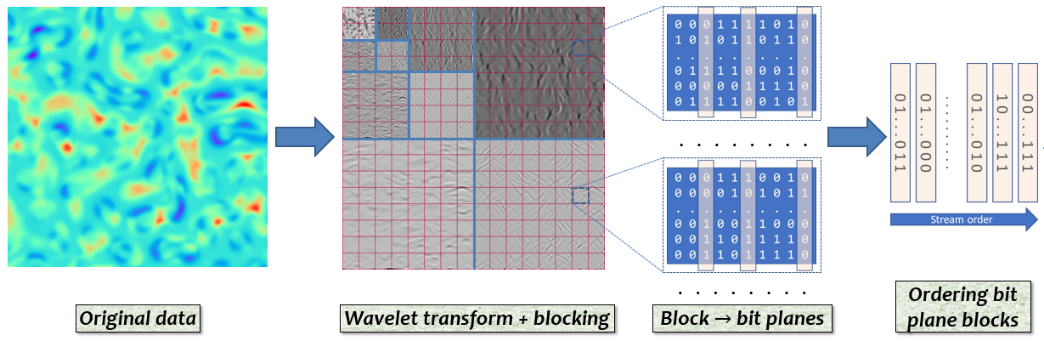
\includegraphics[width=\linewidth]{img/pipeline.png}
\caption{Our data streaming model (in 2D). The input is a regular grid of floating-point samples;
the output is a stream of packets. Different data reduction schemes generate different streams.  The
wavelet subbands are separated by blue lines in the second image, with the coarsest subband at the
top left corner. Although not shown here, quantization and negabinary convesion happen immediately
after wavelet transform. \todo{TODO: revise this figure}}\label{fig:pipeline}
\end{figure}

\begin{table}[!b]
\centering
\begin{tabular}{l l c c}
\toprule
Symbol & Name & Data Dependent & Task Dependent \\
\midrule
\slvl & (\emph{by level}) & \xmark & \xmark\\
\sbit &(\emph{by bit}) & \xmark & \xmark\\
\swav &(\emph{by wavelet norm}) & \xmark & \xmark\\
\smag &(\emph{by magnitude}) & \cmark & \xmark\\
\stkop &(\emph{task-optimized}) & \cmark & \cmark\\
\stksg &(\emph{by signature}) & \cmark/\xmark & \xmark\\
\bottomrule
\end{tabular}\label{tbl:streams}
\caption{We define various types of data streams, including several
data-independent, data-dependent and task-independent, as well as
task-dependent streams. \hb{Duong, \ssig is classified correctly?}\todo{fix
width}}
\end{table}

\subsection{Decomposition of Data into Packets} \label{sec:data-streaming-framework}

Although one way to compare different data reduction strategies is to restrict the techniques to the
same data size and compare data quality, it becomes difficult to enforce consistency. For example,
the amount of change (in data) in one step of multiresolution simplification may be different from
removing one bit in the quantization of every data sample. To avoid such mismatch of units of data
increment/decrement, we model each reduction scheme as a stream of equally sized \emph{packets},
which, we use as as the smallest units of data transfer in our framework. A packet consists of a
relatively small number of bits from a data set. We associate a packet with a resolution level and a
precision level (i.e., bit plane), such that each packet can improve either the resolution or the
precision of data.  In this framework, different data-reduction schemes become different orderings
of packets, called \emph{stream}. Restricting two (or more) data streams to the same number of
packets allows us to perform fair and consistent comparisons.

\para{Packets for Different Resolution Levels.} Although there exist several ways to define the
notion of resolution/scale/frequency, we choose wavelet transform due to the compact support of
their basis functions, which enables spatial adaptivity (i.e., finer resolution in regions that
contain sharp features, at the expense of coarser resolution elsewhere). In particular, we choose
the CDF5/3 discrete wavelet transform~\cite{cdf-wavelets} for its balance between simplicity and
effectiveness at decorrelating the input signal in practice~\cite{jpeg2000}.

A multidimensional wavelet transform can be performed in multiple passes, which partitions the
original domain into \emph{subbands}, each of which can be thought of as a resolution level. One
transform pass (in 3D) creates eight subbands, of which the first is a smoothed, downsampled version
of the original data, and the remaining add fine details in each subset of the dimensions (see
\Cref{fig:pipeline} for a visualization of subbands in 2D). A subsequent transform pass recurses
only on the first subband, creating the next (resolution) level of subbands. We use $l$ $(0 \leq l <
L)$ to index the subbands, with $l = 0$ referring to the coarsest subband and $L$ denoting the
number of subbands. In this paper, we use $L=22$, corresponding to three transform passes in 3D.

\para{Packets for Different Precision Levels.} For creating packets corresponding to different
precision levels, we quantize floating-point wavelet coefficients to $B$-bit signed integers. For
most of the experiments in this paper, $B=16$. This quantization eliminates the exponent bits, such
that every bit (except the sign bit) can be associated with a bit plane $b$ ($0\leq b < B$). To
avoid special treatment of the sign bit, we convert quantized coefficients from two's complement
form to a negabinary form, in which integers are represented in base $-2$, i.e.,
$\sum_{i=0}^{B}{c_i(-2)^i}$ with $c_i\in \{0,1\}$. This transformation increases the number of bit
planes by one, to compensate for the absence of the sign bit. In our convention, the higher indexed
bit planes are less significant.

Precisely, a packet consists of bits on the same bit plane, from a \emph{block} of negabinary
wavelet coefficients. A block is a $[g\times g\times g]$ grid of adjacent coefficients on the same
subband. We let $g$ be a constant ($g=2$ in this paper), so that finer resolution subbands contain
more packets, which presents a tradeoff between packets that provides wider (but coarser) coverage
and packets that provides finer (but more local) details. Every packet comes from a bit plane $b$
and a subband $l$. A packets improves the precision (or resolution) of a region if it comes from a
bit plane (or subband) that has not been streamed before in the region. $g$ is chosen to be larger
than one for performance reason, as in practice, most systems read bits in batches.

\subsection{Data-dependent and Data-independent Streams} \label{sec:static-dynamic-streams}

We model two common data reduction schemes in the literature as \emph{by level} and \emph{by bit
plane} streams. The \emph{by level} stream, \slvl, orders the packets strictly from coarser to finer
resolution levels. Within the same subband, packets follow the row-major order of coefficients and
then bit plane order (from 0 to $B$) within each coefficient. The other common ordering, \emph{by
bit plane}, denoted as \sbit, proceeds strictly from higher ordered to lower ordered bit planes.
Within the same bit plane, packets follow the subband order (from 0 to $L$), and then row-major
order in each subband. The streams \slvl and \sbit are designed to mimic the way data is accessed in
traditional methods that work either in resolution (\slvl) or in precision (\sbit).

Additionally, we define a third stream that combines these two dimensions and refer to it as
\emph{by wavelet norm}, or \swav. This stream orders packets in descending order of weights
$\wwav(p)=2^{B-1-b(p)}\times \norm{\omega_{l(p)}}^2$, where $p$ denotes a packet. The first term
captures the contribution of a bit on bit plane $b(p)$, and the second term captures the
contribution of a wavelet coefficient on subband $l(p)$, where $\omega_{l(p)}$ refers to a wavelet
basis function on subband $l(p)$. In the wavelet representation, a function $f$ is written as a
linear sum of wavelet basis functions $\omega_i$: $f=\sum{c_i\omega_i}$, where $c_i$ are the
coefficients. Since basis functions in the same subband share the same norm, $\wwav(p)$ is simply
the contribution (in $L_2$ norm) of a bit on bit plane $b_p$ and subband $l_p$, to the whole
function $f$. A data-reduction scheme based on \emph{by wavelet norm} was hinted at in~\cite{weiss}.

Another common way to reduce data in the wavelet domain is to leave out coefficients of smallest
magnitudes. We model this scheme with a stream called \emph{by magnitude}, or \smag. Here, the
weight function is $\wmag(p)=\sum_{c\in \text{block}(p)}\norm{c}^2$ (the sum is over all
coefficients in the block that contains packet $p$). If two packets have the same weight, they are
ordered by subband index, and then by bit plane. Unlike \slvl, \sbit, and \swav, the \smag stream is
data dependent because the coefficient magnitudes are not known without the data.

In principle, data-dependent streams are better than data-independent streams because they can
prioritize important packets based on the actual data. However, data-dependent streams are
ill-suited for practical purposes, because the cost of sending position information likely outweighs
any potential benefit. Nevertheless, we study them for various reasons. First, the \emph{by
magnitude} scheme is well known in the literature. Second, the ``best'' data-dependent streams can
serve as a benchmark to evaluate the performance of their data-independent counterparts. Finally, in
addition to being data dependent, streams can also be task dependent (\Cref{sec:data_dep_streams}),
which may provide insights into how data should be queried to perform certain analysis tasks.

\subsection{Data-dependent, Task-optimized Streams} \label{sec:data_dep_streams}

Each analysis task may require a fundamentally different stream for optimal results. Studying such
an ``optimal'' (and data-dependent) stream is important because it not only serves as a benchmark,
but also can provide insights into other, more practical streams for the same task.

Given the original data set $f$ and its reconstructed approximation $\tilde{f}$ using a subset of
packets, let $q$ represent some quantity of interest \footnote{In this paper, we use the terms
``quantity of interest'' and ``task'' interchangeably, with the understanding that, e.g., if the
task is extracting isosurface, then the quantity of interest is the isosurface.}, e.g., histogram,
isosurface, etc., computed on $f$ or $\tilde{f}$. For a given task $q$, a well-defined error metric
$\err(q(\tilde{f}),q(f))$ is needed. Given a data set $f$, a task $q$, and an error metric $\err$,
our goal is to generate an \emph{optimal} (and data-dependent) stream, $\sopt$, for $q$ with respect
to $\err$. We can define $\sopt$ as a stream such that the area under the curve of \err is minimized
for all packets to be streamed. However, this definition is limited in practice because a stream
should be able to terminate at any point and still produce as small an error as possible. Moreover,
the solution to the problem has exponential time complexity.

Instead, we employ a greedy approach to define the optimal stream.  A straightforward greedy
algorithm, however, suffers from the usual limitation of potentially leading to a local optimum. For
example, starting with an all-zero reconstruction $\tilde{f}=0$, and an empty stream, we can
repeatedly append new packets to the stream, which when included in the current $\tilde{f}$, would
minimize $\err$ at every step. Each step might pick a packet that introduces low error, yet
contributes very little to improve the quality of $\tilde{f}$, possibly leading to a nonoptimal
stream at a later point. In order to avoid local minima, we make a modification to this greedy
algorithm, and build the stream backwards. We start with a ``lossless'' $\tilde{f}$ (i.e.,
$\tilde{f}=f$), and at each step we remove the packet that has the least impact on the error $\err$
from $\tilde{f}$. This modification solves the previous problem where less important packets were
added to $\sopt$ too early. Moreover, it ensures that the packets chosen for removal early on are
indeed less important and will be put at the end of $\sopt$.

Unfortunately, such a greedy algorithm is still expensive in practice, as its complexity is
$\mathcal{O}(n^3)$, with $n$ being the total number of packets in the data. The cubic time
complexity comes from the complexity of the 2-level nested loop, multiplied by that of the wavelet
transform and error computation. Considering a small, e.g., $[64 \times 64 \times 64]$ domain, a
block size that spans $2^3$ coefficients, and $16$ bits of quantization, $n$ will be 557056, leading
to prohibitively large numbers. Therefore, we adopt a simplified version of this algorithm, where
only one pass through the set of $n$ packets is needed. In each iteration $i$, we disable (set to
zero) a new packet $p_i$ in $\tilde{f}$, compute and record the incurred error $\err_i$, and then
enable $p_i$ again at the end of iteration $i$. After $n$ iterations, each packet has an associated
weight $\err_i$. The stream $\sopt$, then, is simply the sorted list of packets in decreasing order
of the weights. This simplified algorithm brings the running time from days down to hours, while (by
observation) retaining the same quality for $\sopt$. \Cref{alg:greedy} outlines the approach
described above.

\begin{algorithm}[h]
  \caption{Computing a task-optimized stream}
  \begin{algorithmic}[1]
    \Inputs{
			An original function $f$\\
			An unordered set of $n$ packets $P = \{p_i\}$, produced from $f$\\
			A quantity of interest $q$, and an error function $\err$}
		\Initialize{A set of $n$ weights $\Gamma = \{\gamma_i\}$ }
		\For{each packet $p_i$}
			\State $p_i := 0$
      \State $P \rightarrow$ wavelet coefficients $W$ \\
      		\ \ \ \ \ \ \ \ \ \ \ \ (inverse quantization and inverse negabinary transform)
			\State $W \rightarrow f'$ (inverse wavelet transform)
			\State $\gamma_i := \err(q(f'),q(f))$			
			\State Restore $p_i$
		\EndFor
		\State Sort the $p_i$'s in descending order of $\gamma_i$.
		\Output{The $q$-optimized stream, which is the sorted $P$}
	\end{algorithmic}
	\label{alg:greedy}
\end{algorithm}

\subsection{Stream Signatures} \label{sec:stream-signature}
Unlike data-independent streams, data-dependent streams do not impose a static ordering of packets.
To concisely represent and characterize the dynamic ordering of data-dependent streams, we introduce
the notion of a \emph{stream signature}. Any stream can be represented with respect to the
two-dimensional space of resolution (subbands) and precision (bit planes), i.e., \mbox{$
\Sigma_{L,B}=\{(l,b)\ |\ 0\leq l < L,\ 0\leq b < B\}$.}

Given a stream, we define its signature $\sgn_{L,B}$ as an $L \times B$ matrix, where each $(l,b)$
element is associated with $P_{l,b}$---the set of packets belonging to subband $l$ and bit plane
$b$. In particular, $\sgn(l,b)$ is an integer in the range $[0, B\times L)$, and indicates, on
average, the position at which packet $P_{l,b}$ appears in the given stream. For example, the
signature $\sgn=\bigl[ \begin{smallmatrix}0 & 1 & 4\\ 2 & 3 & 5\end{smallmatrix}\bigr]$ indicates
that the stream begins with packets that lie on the first bit plane of the first subband, as
$\sgn(0,0)=0$. Those are followed by packets on the second bit plane of the first subband
($\sgn(0,1)=1$), and then the first bit plane of the second subband ($\sgn(1,0)=2$), and finally,
the third bit plane of the second subband ($\sgn(1,2)=5$). Thus, a stream's signature shows how the
stream traverses the space $\Sigma_{L,B}$, and highlights the different resolution-versus-precision
tradeoffs among streams, especially among $\sopt$ streams optimized for different tasks.
In~\Cref{fig:example-signatures} we visualize the signatures of \sbit, \slvl, and \swav, defined
in~\Cref{sec:data-streaming-framework}.

To compute a stream signature, we partition the whole domain (not individual subbands) into several
\emph{regions}, compute one signature per region, and average these local signatures. It is only
when packets are relatively well localized that their relative ordering in the $\Sigma_{L,B}$ space
becomes meaningful. For example, a packet at one corner of the domain may be streamed before one at
an opposite corner, but this fact contains no useful information. We define a region to be the
spatial volume that is covered by a packet in the coarsest subband. Algorithm~\ref{alg:signature}
lists the steps of our approach.

\begin{algorithm}[h]
  \caption{Computing a stream signature}
  \begin{algorithmic}[1]
    \Inputs{
			A stream $P=\{p_i\}$\\}
		\Initialize{Per-region signature matrix $A_r:= 0$\\
		Global signature matrix $A := 0$}
		\For{each packet $p_i$ in $P$}
			\State Let $r$, $b$, $l$ be the region, bit plane, and subband that $p_i$ belongs
			\State $A_r(l,b) := A_r(l,b)+i$
		\EndFor
		\For{each region $r$}
			\State Sort the elements of $A_r$
			\State Assign each element of $A_r$ its index after sorting
			\State $A := A+A_r$
		\EndFor
		\State Sort the elements of $A$
		\State Assign each element of $A$ its index after sorting
		\Output{The signature matrix $A$}
	\end{algorithmic}
	\label{alg:signature}
\end{algorithm}

Finally, a signature can be used to construct a stream which lies between data-independent and
data-dependent streams, denoted generically as $\ssig$. This construction is done by iterating
through each element $\sgn(l,b)$ in ascending order, and adding to the end of $\ssig$ all the
packets in $P_{l,b}$. An $\ssig$ captures the behavior (in the $\Sigma_{L,B}$ space) of the stream
it derives from, but is stripped from any spatial adaptivity. Hence $\ssig$ can serve as a bridge
when comparing the resolution-versus-precision tradeoffs between data-independent and data-dependent
streams.

\begin{figure}[t]
\centering
 \subcaptionbox{\label{fig:by-level-signature}\emph{by level} (\slvl)}{{
\includegraphics[width=0.32\linewidth]{SIG-(STATIC)-(BY-LEVEL)-(rmse)}}}
 \subcaptionbox{\label{fig:rmse:diffisivity}\emph{by bit plane} (\sbit)}{{
\includegraphics[width=0.32\linewidth]{SIG-(STATIC)-(BY-BIT-PLANE)-(rmse)}}}
 \subcaptionbox{\label{fig:rmse:plasma}\emph{by wavelet norm} (\swav)}{ {
\includegraphics[width=0.32\linewidth]{SIG-(STATIC)-(BY-WAVELET-NORM)-(rmse)}}}
\caption{Renderings of signatures for \slvl, \sbit, and \swav in 2D. Each signature is a $10\times
17$ image, corresponding to $10$ subbands and $17$ bit planes. Each $(l,b)$ ``cell'' contains a
unique value from $0$ to $169$, indicating its ``priority'' in stream, and which is mapped through a
linear blue color map ($0$ is mapped to the brightest blue). It is clear that the \slvl streams bits
by resolution (from top to bottom), \sbit streams by precision (from left to right), while \swav
mixes precision and resolution.}
\label{fig:example-signatures}
\end{figure}

\section{Analysis tasks}
\label{sec:analysis-tasks}

In this section, we study a range of fundamental analysis tasks, namely function reconstruction
(Section~\ref{sec:rmse-optimized}), gradient computation (Section~\ref{sec:gradient}), Laplacian
computation (Section~\ref{sec:laplacian}), histogram computation (Section~\ref{sec:histogram}), and
isocontour extraction (Section~\ref{sec:isocontour}). For each task, we define an error metric $E$
(see Section~\ref{sec:data_dep_streams}) that is the basis for evaluating a stream's performance.
Algorithm~\ref{alg:greedy} is used to compute a greedy stream optimized for the task at hand, in
terms of minimizing the relevant $E$ at every point. Each analysis task potentially requires a
fundamentally different stream for optimal results. Therefore, the goal is to distill the core
characteristics of these optimized streams. To accomplish this goal, we define and make use of a
concept named \emph{stream signature} (Section~\ref{sec:stream-signature}). The signature of a
stream is a small matrix that encodes the stream's ``preferences'' in terms of
precision-versus-resolution tradeoffs. As such, the signature not only reveals the characteristics
of a stream, but can also be used in practice to ``steer'' streaming in a way that is optimized for
the task at hand.

\subsection{Stream signatures}
\label{sec:stream-signature}

To analyze the core characteristics of a stream, we introduce the concept of a \emph{stream
signature}. A signature is a $\bar{l} \times \bar{b}$ matrix, with $\bar{b}$ being the number of bit
planes, and $\bar{l}$ the number of wavelet subbands. The $(l,b)$ element of the matrix is
associated with chunks belonging in subband $l$ and bit plane $b$ , and contains an integer value in
the range $[0,\bar{b}\times \bar{l})$. This value indicates, on average, the position in which
chunks associated with that element appear in the stream, relative to chunks associated with other
elements. For example, the signature  $A=\bigl[
\begin{smallmatrix}0 & 1 & 4\\ 2 & 3 & 5\end{smallmatrix}\bigr]$. This signature conveys the
information that the most important chunks lie on the first bit plane of the first subband
($A_{0,0}=0$), followed by chunks lying on the second bit plane of the first subband ($A_{0,1}=1$),
then the first bit plane of the second subband ($A_{1,0}=2$), and so on.

To compute a stream signature, we partition the whole domain into several \emph{regions}, compute
one signature per region, then sum all the per-region signatures. Partitioning is needed since it is
only meaningful to compute the relative ordering of chunks if they come from the the same (``small''
enough) region. For example, a chunk at one corner of the domain can be streamed before another
chunk at an opposite corner, but this fact contains no useful information. We want a region to be as
small as possible, and define a region to be the spatial volume/area that is covered by a chunk in
the coarsest subband. So, the total number of regions is the same as the number of chunks in the
coarsest subband. Note that regions exist in the global domain, as they are not confined to
individual subbands. Ideally, the global signature should retain information from all the per-region
signatures, but due to space constraints, we have chosen to condense all the local signatures by
summing them into one signature. This choice results in signatures that are less meaningful for data
that contains a high degree of spatial variability. We have found, however, that this choice works
well for the various data sets used in this paper. If signatures are deemed useful enough to be
deployed in practice, a more sophisticated ``compression'' of the signature stack might be necessary
for the best results.

The following algorithm computes a stream signature.

\begin{algorithm}[h]
  \caption{Computing a stream signature}
  \begin{algorithmic}[1]
    \Inputs{
			A stream $C$\\}
		\Initialize{A set of weights $\Gamma = \{\gamma_i\}, i\in \{1,\dots,n\}$ }
		\For{$i$ = $1$ to $n$}
			\State $c_i \gets 0$
      \State Back-transform $C$ to produce a set of wavelet coefficients $W$
			\State Perform inverse wavelet transform on $W$ to produce $f'$
			\State $\gamma_i \gets E(Q(f'),Q(f))$			
			\State Restore $c_i$
		\EndFor
		\State Sort the $c_i$'s in descending order of $\gamma_i$.
		\Output{The $Q$-optimized stream, which is the sorted $C$}
	\end{algorithmic}
	\label{alg:greedy}
\end{algorithm}

TODO: example signatures for the by bit plane, by level, by wavelet norm

\subsection{Function reconstruction}
\label{sec:rmse-optimized}

The most fundamental task is that of reconstructing the function itself (i.e., $Q$ is the identity
map), using a common error metric such as the root-mean-square error (RMSE). For each data set, we
use the aforementioned $O(n)$ greedy algorithm to construct an \emph{rmse-optimized} stream. In
Section \ref{sec:motivation} we have seen that the \emph{by wavelet norm} performs the best among
the data-agnostic streams with regards to RMSE. To see how the \emph{rmse-optimized} stream, which
is data-dependent, compares to the data-agnostic streams, we plot all four streams together in
Figure \ref{fig:rmse-optimized}. It can be seen that the difference between \emph{by wavelet norm}
and \emph{rmse-optimized} is negligible in most cases. This result is expected, because \emph{by
wavelet norm} and \emph{rmse-optimized} both order the chunks according to their contribution to in
the $L_2$ sense, with \emph{rmse-optimized} also taking into account the actual values of the bits.
This difference has little effect in this case, because, as leading zero bits are removed, the rest
of the bits (of the wavelet coefficients) are known to be distributed approximately uniformly among
$0$ and $1$ for wavelet coefficients [CITE]. 

Among the static streams, \emph{by level} performs poorly compared to \emph{by bit plane} and
\emph{by wavelet norm}. This is because, in the $L_2$ norm, low-ordered bits or coarse-level
coefficients contribute little compared to high-ordered bits of fine-level coefficients. This
difference in contribution is magnified when the data contains fine-scale features, as is the case
for the \emph{plasma} data set. In Figure \ref{fig:rmse-rendering}, we render this field at 0.74
bits per sample for all three streams, and compare these rendering with that of the groundtruth
data. \emph{by level} results in heavy artifacts that are not seen by \emph{by bit plane} and
\emph{by wavelet norm}. \emph{by wavelet norm} performs slightly better than \emph{by bit plane}
here and in all other cases. These results suggest that in practice, \emph{by wavelet norm} is a
near-optimal way to stream data that minimizes root-mean-square errors, regardless of the data.

\begin{figure}[h]
  \centering
	\subcaptionbox{Boiler}
  {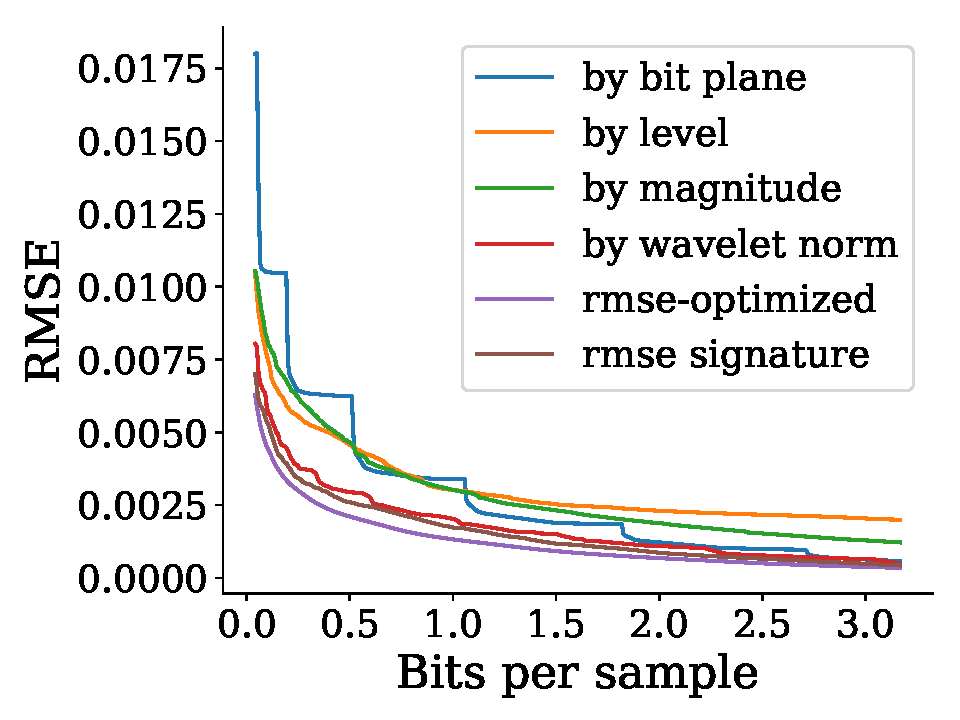
\includegraphics[width=0.48\linewidth]{img/rmse/rmse-optimized-boiler.pdf}}
	\subcaptionbox{Diffusivity}
 	{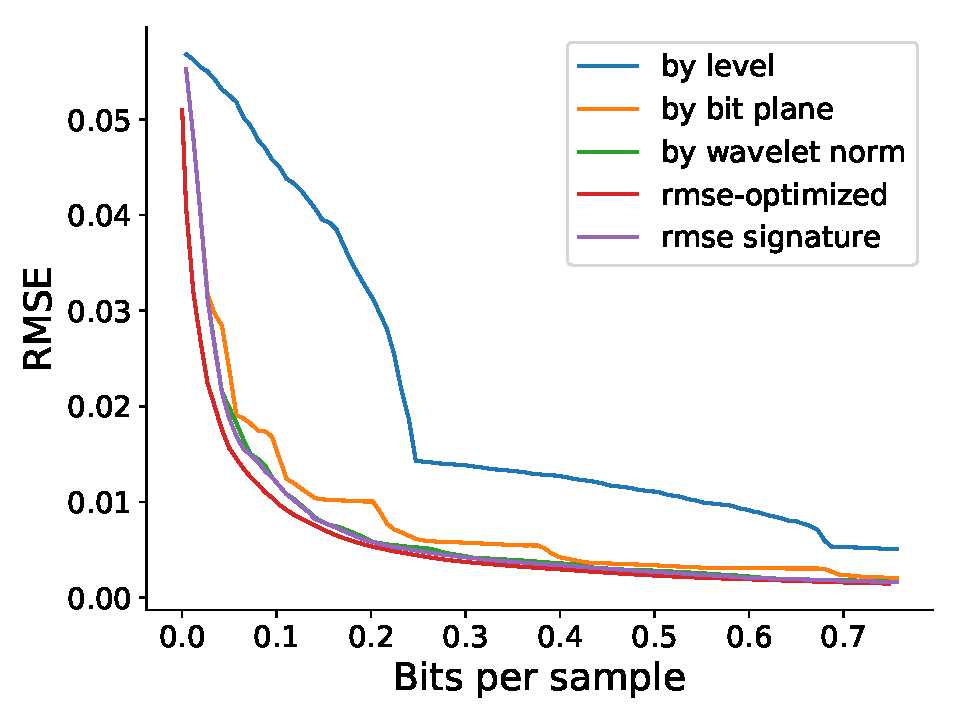
\includegraphics[width=0.48\linewidth]{img/rmse/rmse-optimized-diffusivity.pdf}}
	\subcaptionbox{Euler}
 	{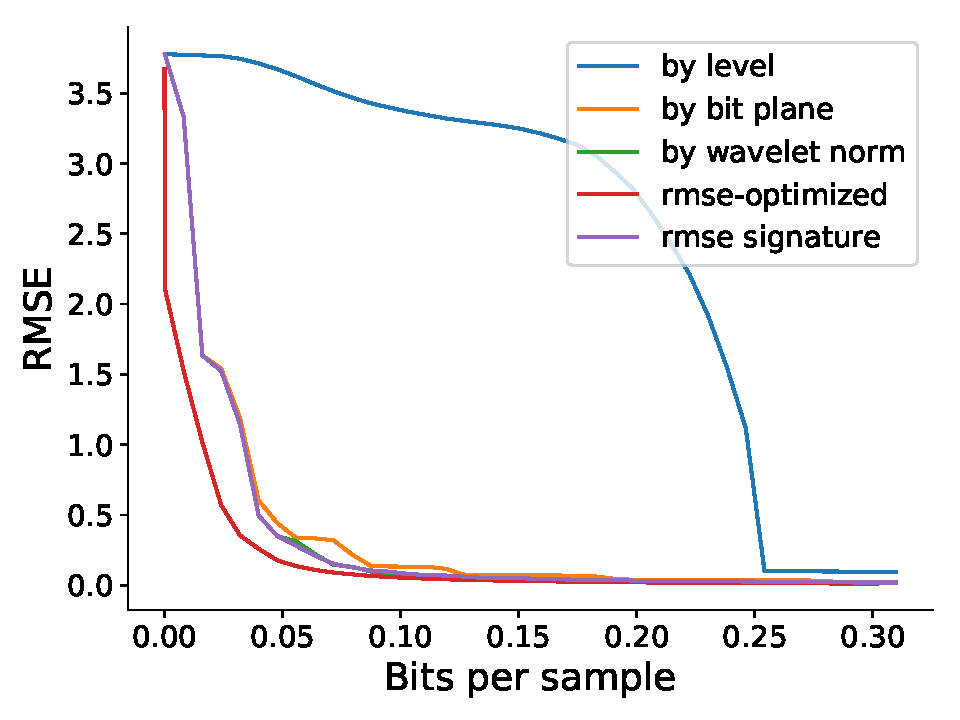
\includegraphics[width=0.48\linewidth]{img/rmse/rmse-optimized-euler.pdf}}
	\subcaptionbox{Turbulence}
 	{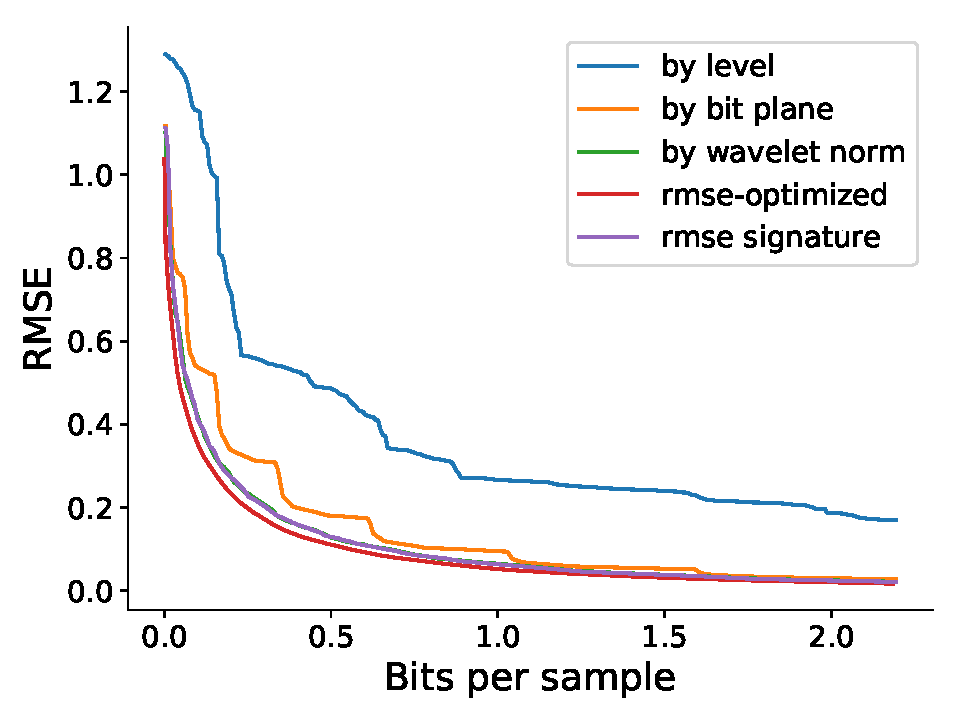
\includegraphics[width=0.48\linewidth]{img/rmse/rmse-optimized-turbulence.pdf}}
	\subcaptionbox{Plasma}
 	{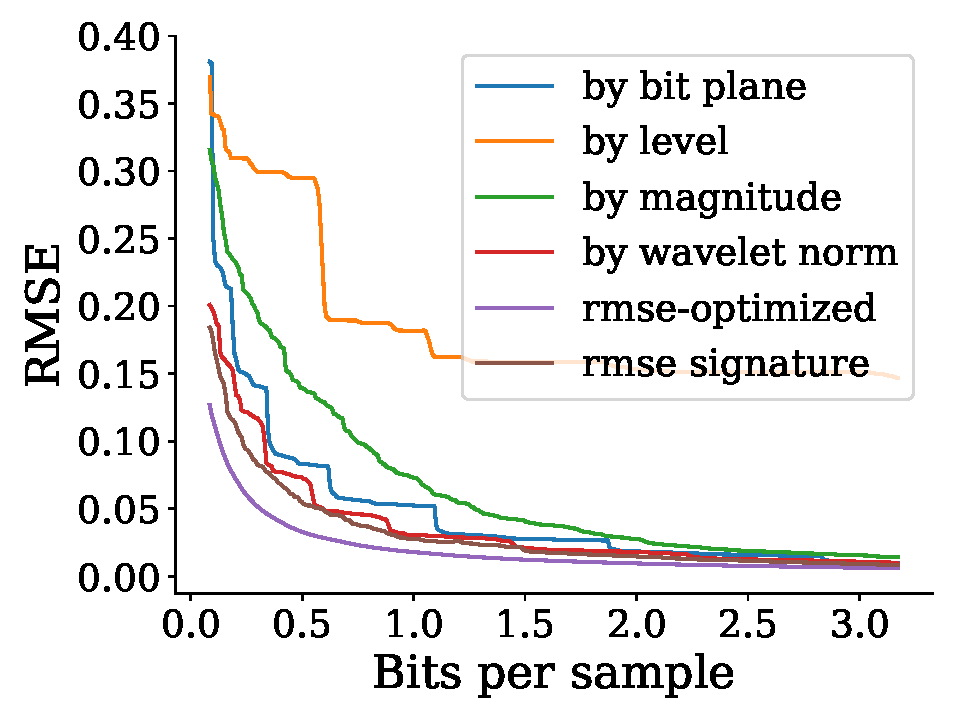
\includegraphics[width=0.48\linewidth]{img/rmse/rmse-optimized-plasma.pdf}}
	\subcaptionbox{Velocity-z}
 	{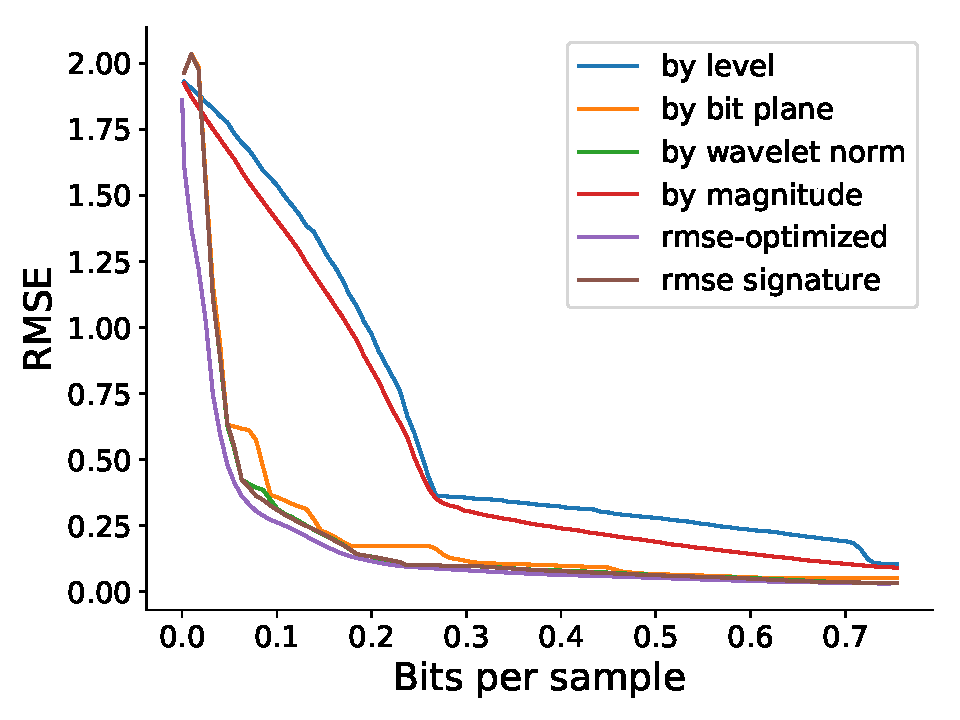
\includegraphics[width=0.48\linewidth]{img/rmse/rmse-optimized-velocityz.pdf}}
 	\caption{Root-mean-square error of reconstructed functions for the three data-agnostic streams
 	defined in Section \ref{sec:motivation}, and the \emph{rmse-optimized} stream. Lower is better.
 	The streams are truncated to highlight the differences, without omitting important information.
 	\emph{rmse-optimized} performs best, followed closely by \emph{by wavelet norm} and \emph{by bit
 	plane}.}
 	\label{fig:rmse-optimized}
\end{figure}

\begin{figure}[h]
	\centering
	{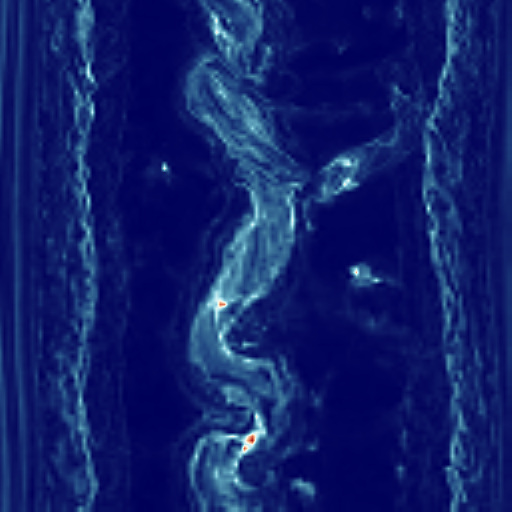
\includegraphics[width=0.24\linewidth]{img/rmse/plasma_curr_func2.png}}
	{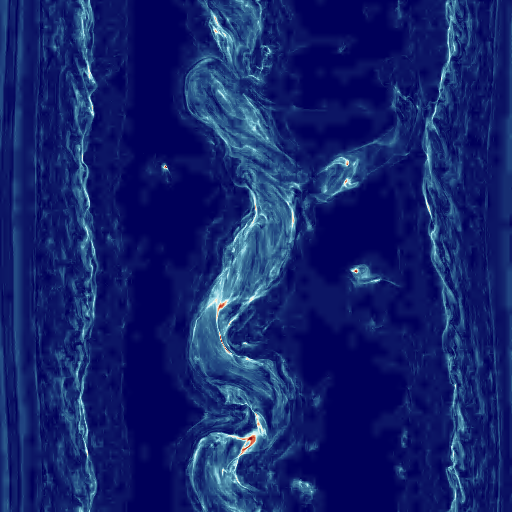
\includegraphics[width=0.24\linewidth]{img/rmse/plasma_curr_func1.png}}
	{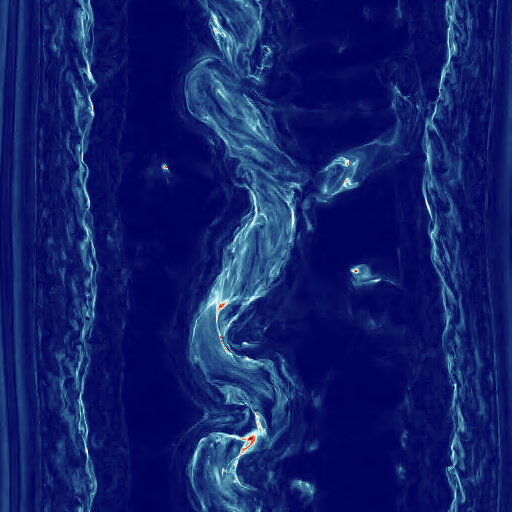
\includegraphics[width=0.24\linewidth]{img/rmse/plasma_curr_func0.png}}
	{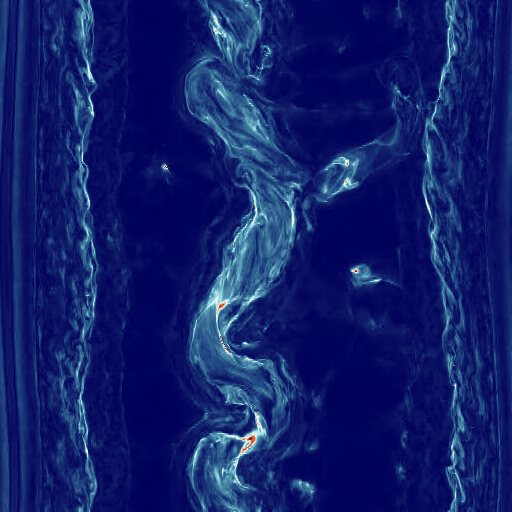
\includegraphics[width=0.24\linewidth]{img/rmse/signature_curr_func0.png}}
	{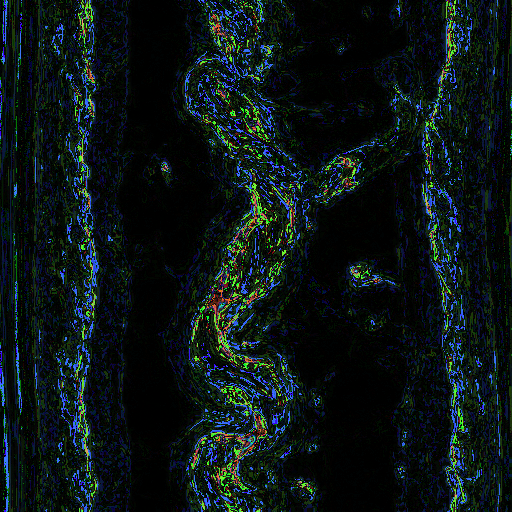
\includegraphics[width=0.24\linewidth]{img/rmse/plasma_curr_func2_diff.png}}
	{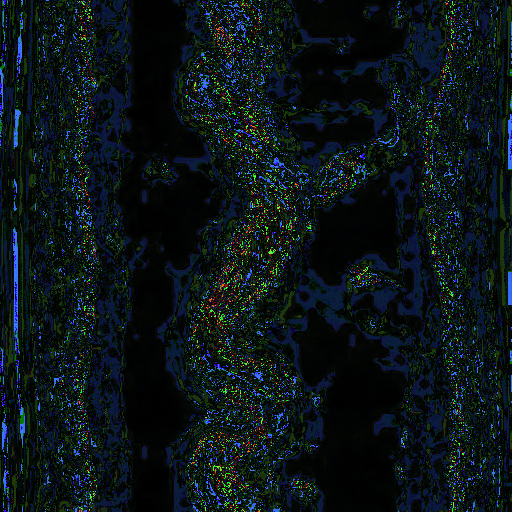
\includegraphics[width=0.24\linewidth]{img/rmse/plasma_curr_func1_diff.png}}
	{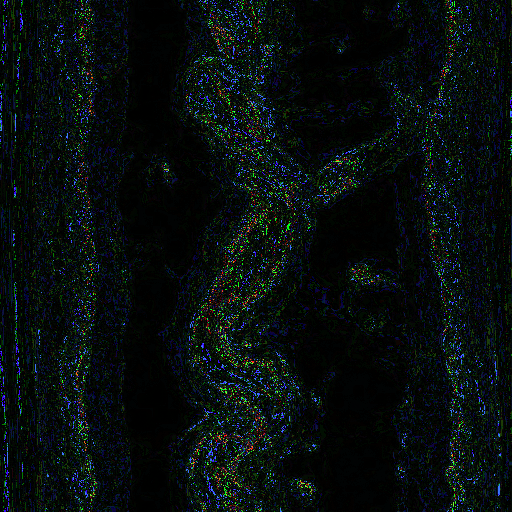
\includegraphics[width=0.24\linewidth]{img/rmse/plasma_curr_func0_diff.png}}
	{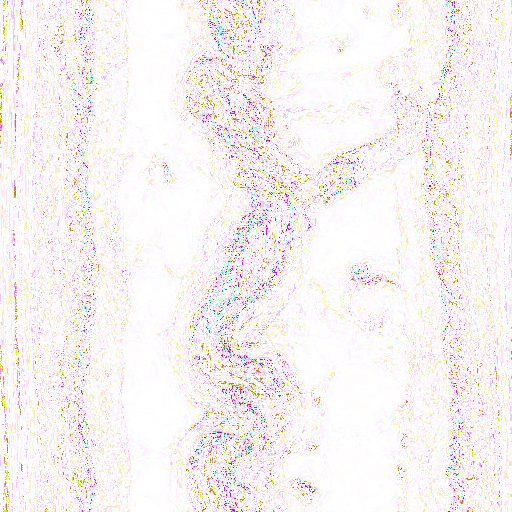
\includegraphics[width=0.24\linewidth]{img/rmse/signature_curr_func0_diff.png}}
	
	\caption{Top row:	renderings of the \emph{plasma} function at 0.74 bps. From left to right:
	\emph{by level}, \emph{by bit plane}, \emph{by wavelet norm}, and ground-truth. Bottom row:
	difference (XOR) of the reconstructed images (in respective order) from the groundtruth image,
	brighter pixels mean higher errors. The \emph{by wavelet norm} provides the most accurate
	function, followed closely by
	\emph{by bit plane}.}
 	\label{fig:rmse-rendering}
\end{figure}

\begin{figure}[h]
	\centering
	{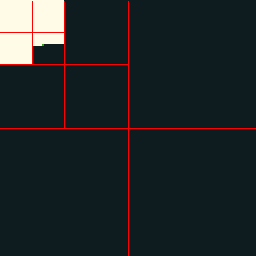
\includegraphics[width=0.24\linewidth]{img/rmse/rmse-precision-dist-by-level.png}}
	{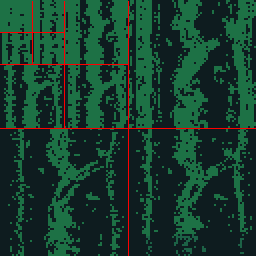
\includegraphics[width=0.24\linewidth]{img/rmse/rmse-precision-by-bit-plane.png}}
	{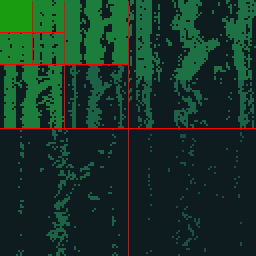
\includegraphics[width=0.24\linewidth]{img/rmse/rmse-precision-dist-by-wavelet-norm.png}}
	{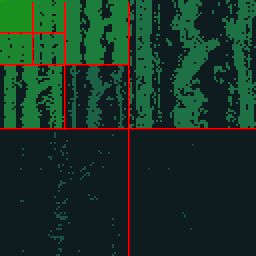
\includegraphics[width=0.24\linewidth]{img/rmse/rmse-precision-signature.png}}
	
	\caption{Precision distribution, plasma, 0.74 bps.}
 	\label{fig:rmse-rendering}
\end{figure}

\subsection{Derivative Computation} \label{sec:derivatives}

Computation of derivative-based quantities is important in data analysis. In this paper, derivatives
are always computed using finite differences, which is common in practice. We use 32 bits for
quantization in this section to ensure enough precision for finite differences, as compared to 16
bits for other experiments. We always compute finite differences on the finest resolution grid to
avoid computing distances between quantities defined on grids of different resolutions.

\subsubsection{Gradient Computation} \label{sec:gradient}

\begin{figure*}[t]
\centering
\subcaptionbox{\emph{boiler}}{%
{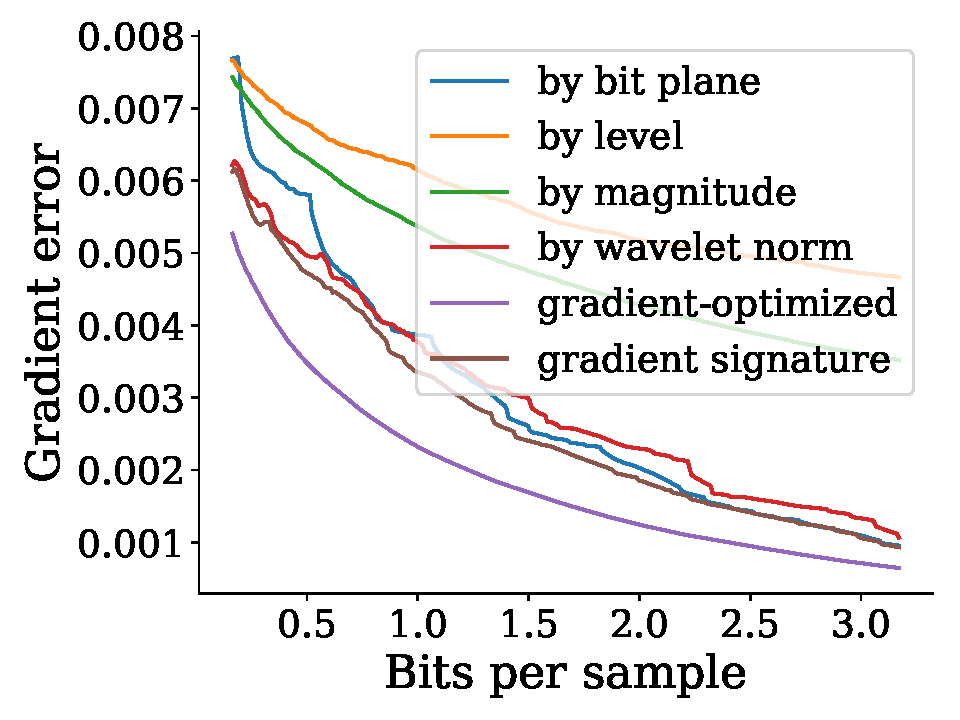
\includegraphics[width=0.24\linewidth]{gradient/gradient-optimized-boiler}}}
\subcaptionbox{\emph{diffusivity}}{%
{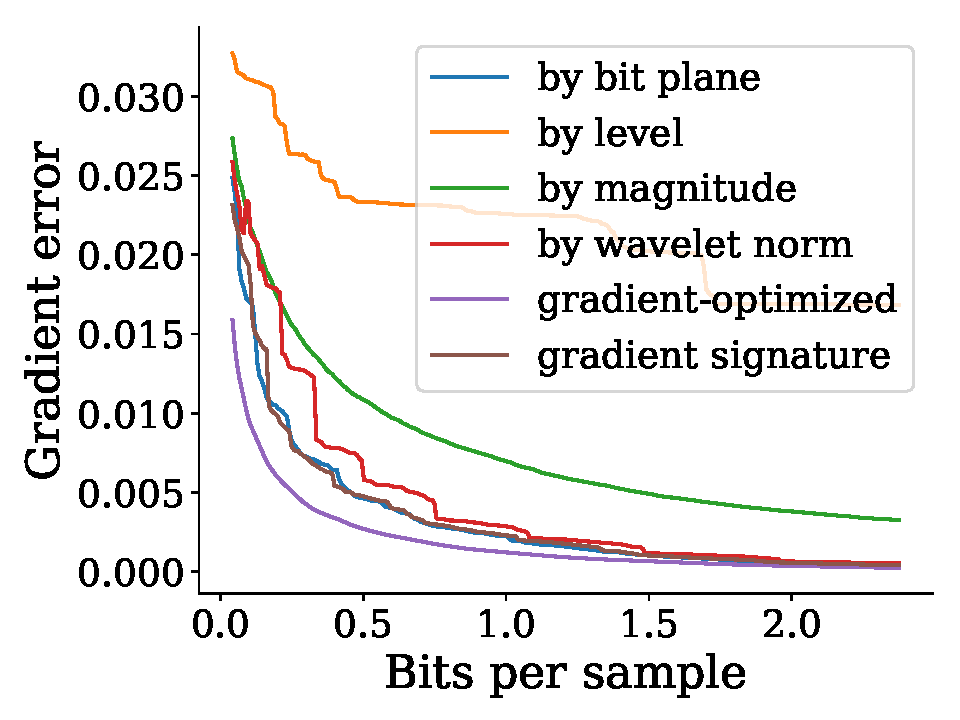
\includegraphics[width=0.24\linewidth]{gradient/gradient-optimized-diffusivity}}}
\subcaptionbox{\emph{turbulence}}{%
{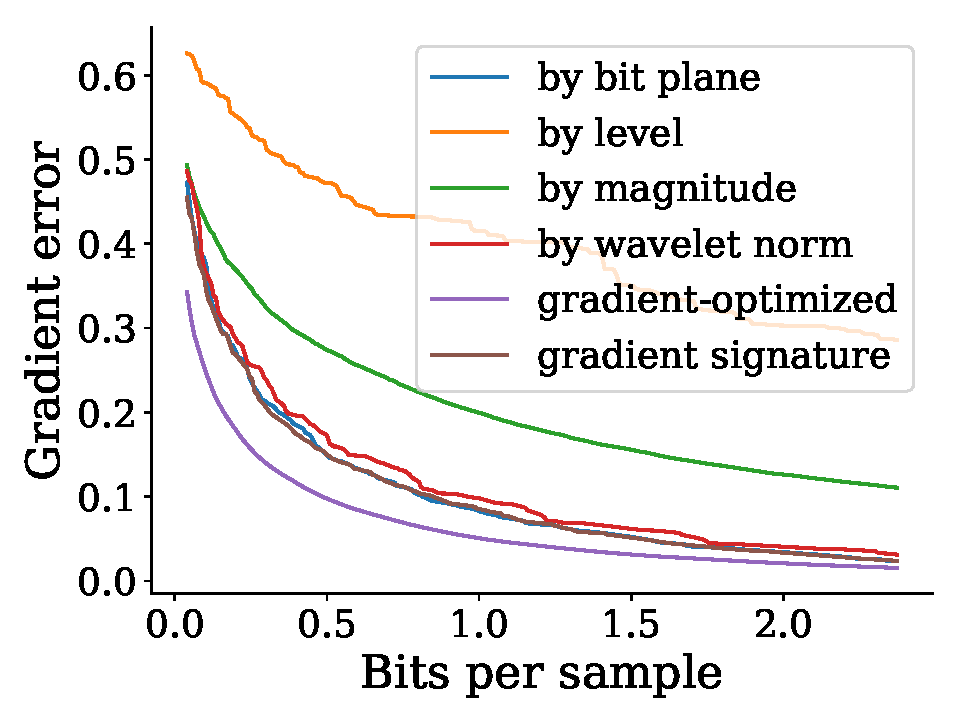
\includegraphics[width=0.24\linewidth]{gradient/gradient-optimized-turbulence}}}
\subcaptionbox{\emph{pressure}}{%
{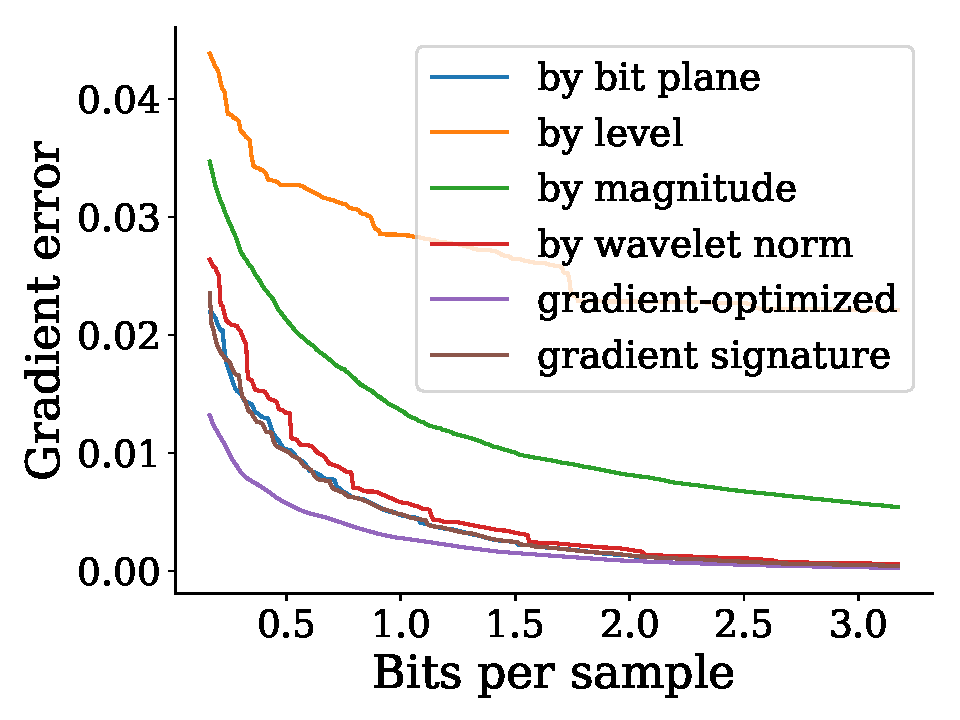
\includegraphics[width=0.24\linewidth]{gradient/gradient-optimized-pressure}}} 
\caption{Gradient error of reconstructed functions. Lower gradient error is better. Leading zero
packets are removed, and the plots are truncated in the same way as in~\Cref{fig:rmse-optimized}.
The trend in error, in all cases, is $\sgop < \sgsg \approx \sbit < \swav < \smag < \slvl$.}
\label{fig:gradient-error-comparison}
\vspace{1em}

\centering
\subcaptionbox{\emph{by level} (\slvl)}{%
{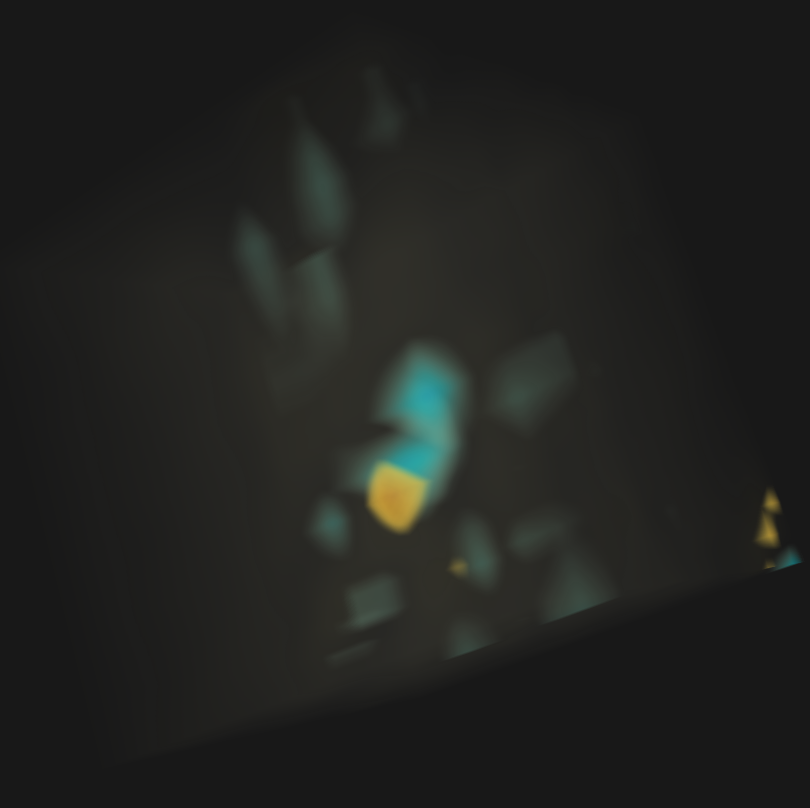
\includegraphics[width=0.16\linewidth]{gradient/gradient-turbulence-level}}}
\subcaptionbox{\emph{by bit plane} (\sbit)}{%
{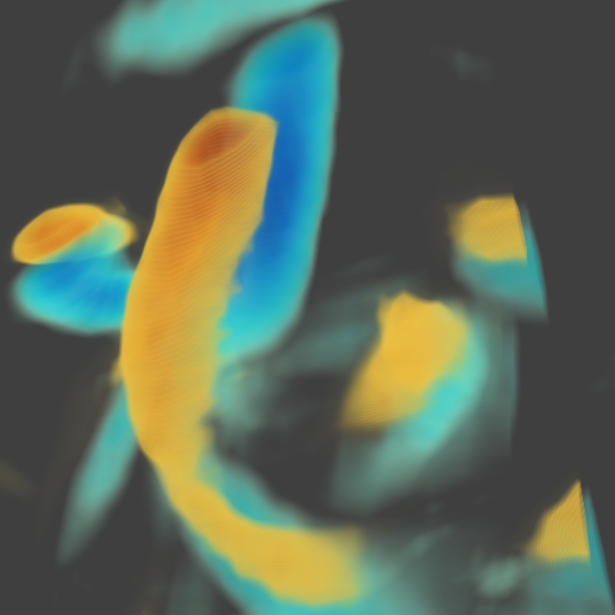
\includegraphics[width=0.16\linewidth]{gradient/gradient-turbulence-bit-plane}}}
\subcaptionbox{\emph{by wavelet norm} (\swav)}{%
{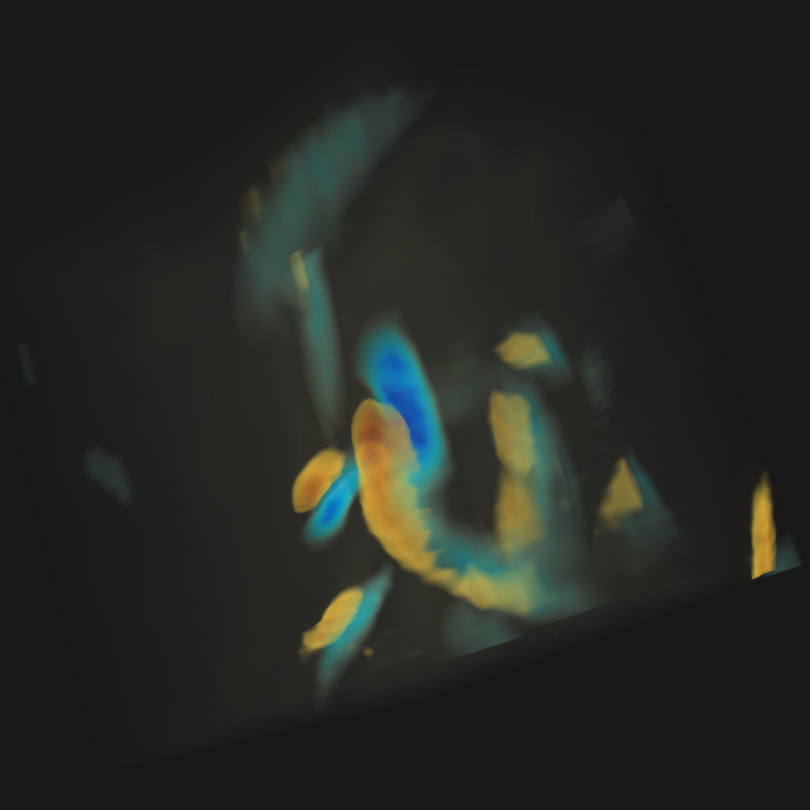
\includegraphics[width=0.16\linewidth]{gradient/gradient-turbulence-wavelet-norm}}}
\subcaptionbox{\emph{by magnitude} (\smag)}{%
{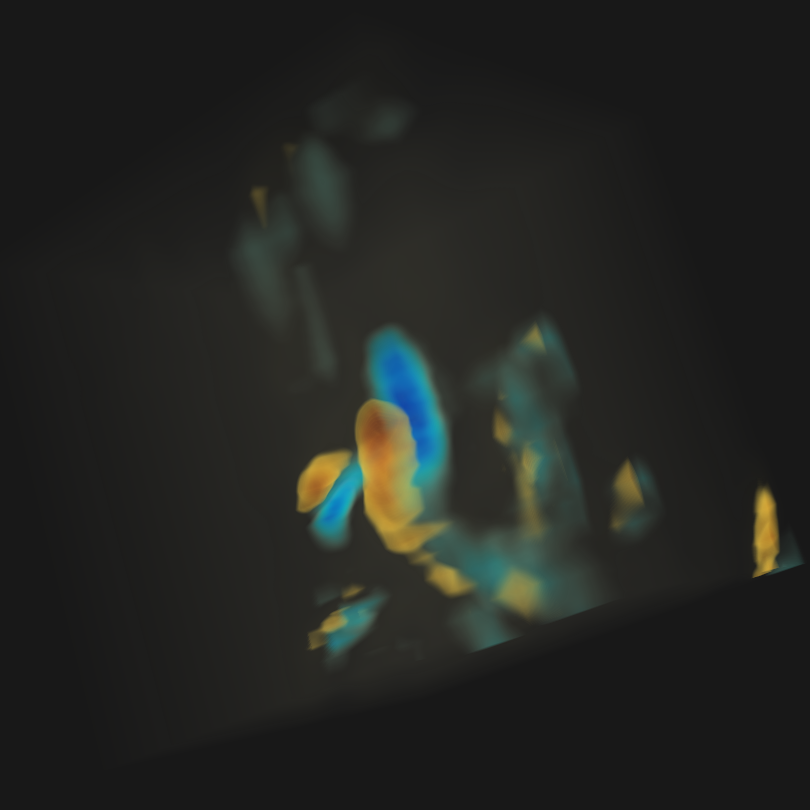
\includegraphics[width=0.16\linewidth]{gradient/gradient-turbulence-magnitude}}}
\subcaptionbox{\emph{by signature} (\sgsg)}{%
{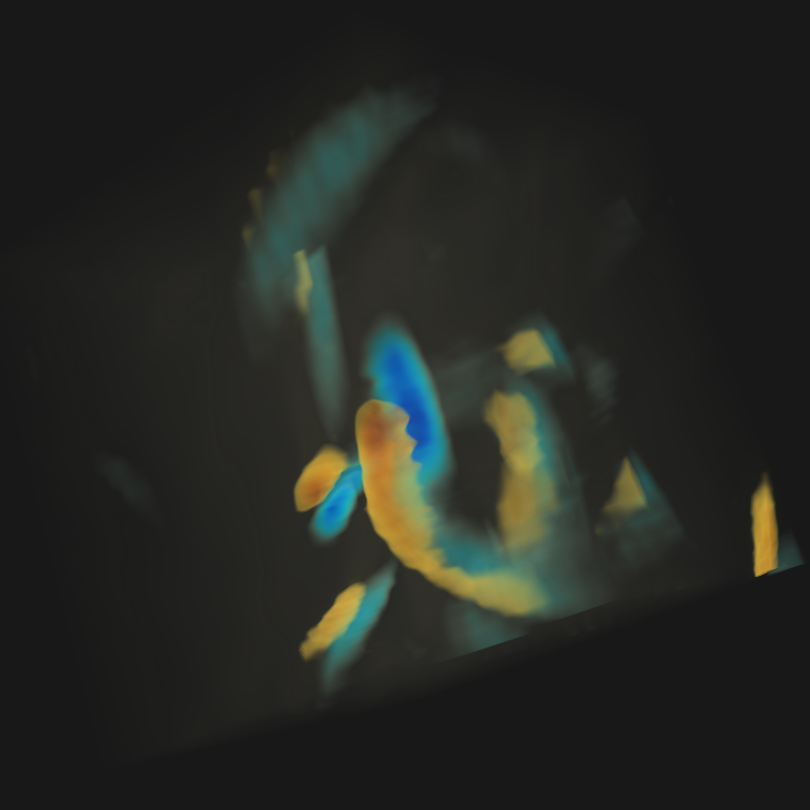
\includegraphics[width=0.16\linewidth]{gradient/gradient-turbulence-signature.png}}}
\subcaptionbox{\emph{ground truth}}{%
{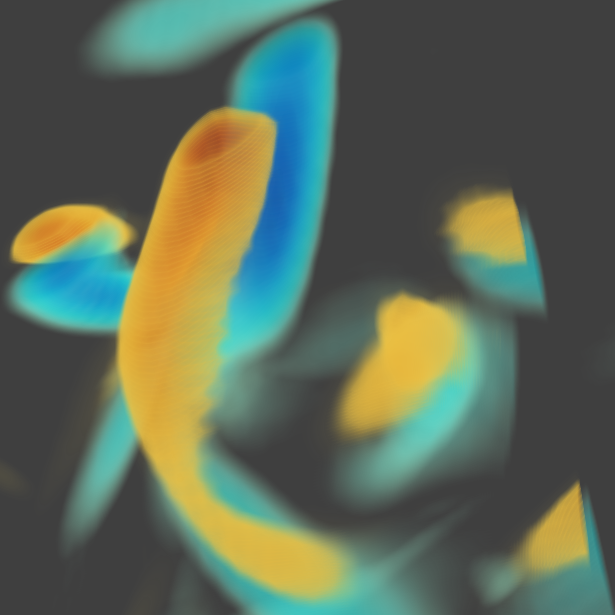
\includegraphics[width=0.16\linewidth]{gradient/gradient-turbulence-groundtruth.png}}}
\caption{$x$-component of the ($64^3$) gradient field of \emph{turbulence}, reconstructed at 0.5
bps. The gradient field produced by \sbit is more accurate than one produced by \swav, and slightly
more accurate than one produced by \sgsg (compare orange features).}
\label{fig:gradient-rendering-diff}
\end{figure*}

\begin{figure}[h]
\centering
\subcaptionbox{\emph{by bit plane} (\sbit)}{
{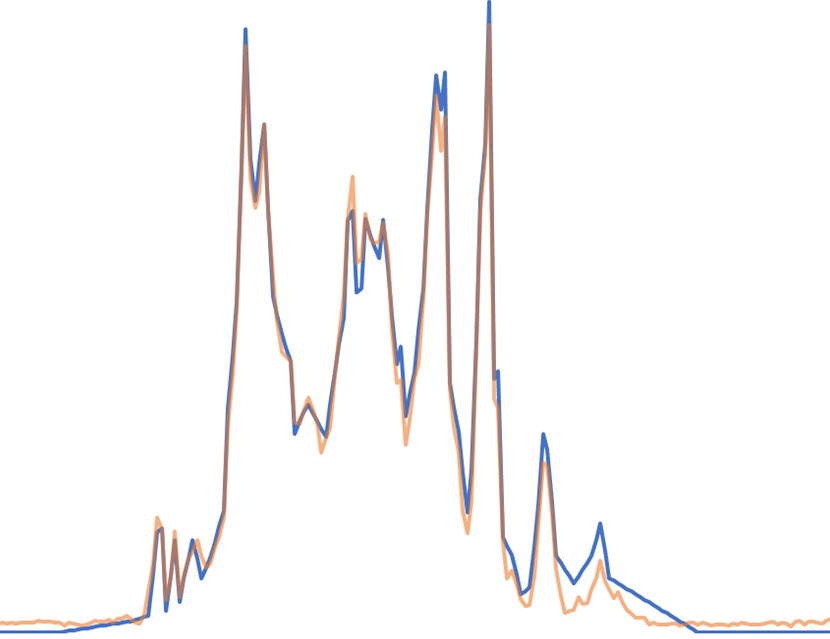
\includegraphics[width=0.48\linewidth]{gradient/gradient-bit-plane}}} 
\subcaptionbox{\emph{by wavelet norm} (\swav)}{
{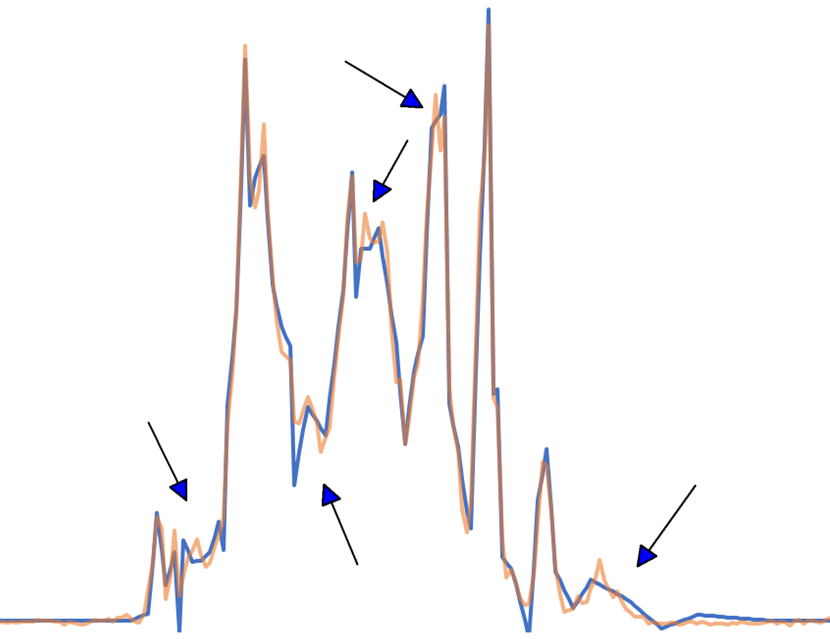
\includegraphics[width=0.48\linewidth]{gradient/gradient-wavelet-norm}}}
\caption{A 1D line extracted from \emph{plasma}, and reconstructed using \sbit and \swav at 0.6 bps.
The original data is in orange and the reconstructions are in blue. \swav captures well the function
values in low-gradient regions, where \sbit struggles (red arrows). However, \sbit retains the shape
of the original function well in areas of both low and high gradients, where \swav instead produces
smooth approximations (blue arrows). \sbit therefore is better for derivative computations, where a
function's shape (or its relative values) matters more than its absolute values.}
\label{fig:bit-plane-vs-wavelet-norm-gradient}
\end{figure}

Given a function $f$ defined on a grid, its gradient at a grid point \mbox{$\x = (x,y,z)$} is the
vector $\nabla f(\x) = \left(\frac{\partial f}{\partial x}, \frac{\partial f}{\partial y},
\frac{\partial f}{\partial z}\right)$. We use a five-point stencil to compute the gradient, i.e.,
$\frac{\partial f}{\partial x} \approx \frac{1}{12}f(x-2,y,z) - \frac{2}{3}f(x-1,y,z) +
\frac{2}{3}f(x+1,y,z) - \frac{1}{12}f(x+2,y,z)$. The error between a gradient field $\nabla f$, and
its low-bit-rate approximation $\nabla
\tilde{f}$, is defined as $\err(\nabla \tilde{f}, \nabla f) = \sqrt{\frac{1}{N}
\sum_{i=1}^{N}{\norm{\nabla \tilde{f}(\x_i)-\nabla f(\x_i)}^2}}$. Using~\Cref{alg:greedy}, we
compute a \emph{gradient-optimized} stream, \sgop, i.e., a stream that minimizes the difference
between the reconstructed gradient field and the original gradient field.

\Cref{fig:gradient-error-comparison} shows the gradient error incurred by different streams for four
data sets. In general, we observe the ordering of performance (from best to worst) as: \sgop, \sgsg,
\sbit, \swav, \smag, \slvl. This ordering can also be seen in~\Cref{fig:gradient-rendering-diff},
where the $x$-component of the gradient field for \emph{tuburlence} is rendered at 0.5 bps. Unlike
the RMSE case, \sbit produces better approximations of the gradient field compared to \swav.

We further investigate this difference by extracting a 1D line from the \emph{plasma} data set and
reconstructing the function using \sbit and \swav at 0.6 bps
(\Cref{fig:bit-plane-vs-wavelet-norm-gradient}). Because the coarse-scale coefficients in \sbit are
approximated at low precision, the reconstruction from \sbit is inaccurate in areas of low
gradients. In contrast, \swav's reconstruction is accurate in low-gradient areas, but lacks the
resolution to resolve the high-gradient areas, because \swav frequently intersperses bits that
improve resolution with bits that improve precision, unlike \sbit, which always streams bits that
improve resolution first. Therefore, \swav tends to produce a ``smoother'' reconstruction that
\emph{on average} (e.g., in terms of RMSE) is close to the original function. \sbit, on the other
hand, tends to capture well the function's shape (due to fine-scale bits), but the whole function
can be ``shifted'' slightly due to the lack of precision in coarse-scale coefficients. However, the
error caused by this shifting reduces significantly when taking the gradient, which cancels any
constant shift. \sbit, therefore, works better than \swav for gradient computation, because it is
better able to retain sharp features.

\sgop again outperforms the rest of the streams. \slvl and \smag perform poorly for gradient
computation, lacking the resolution to capture sharp features. \sgsg closely follows \sbit in
performance (it is slightly better than \sbit for \emph{boiler} at very low bit rates). These
results suggest that while \swav is the best among the data-independent streams when optimizing for
RMSE, \sbit is better for gradient computation.

\subsubsection{Laplacian Computation}\label{sec:laplacian}

\begin{figure*}[h]
\centering
\subcaptionbox{\emph{boiler}}
{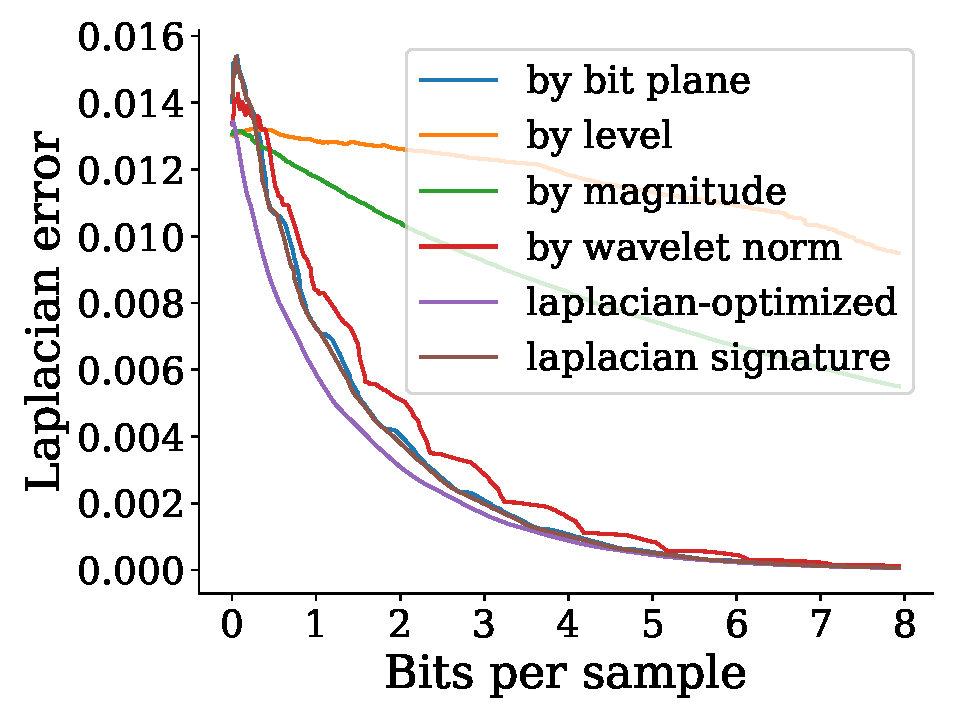
\includegraphics[width=0.24\linewidth]{laplacian/laplacian-optimized-boiler}}
\subcaptionbox{\emph{diffusivity}}
{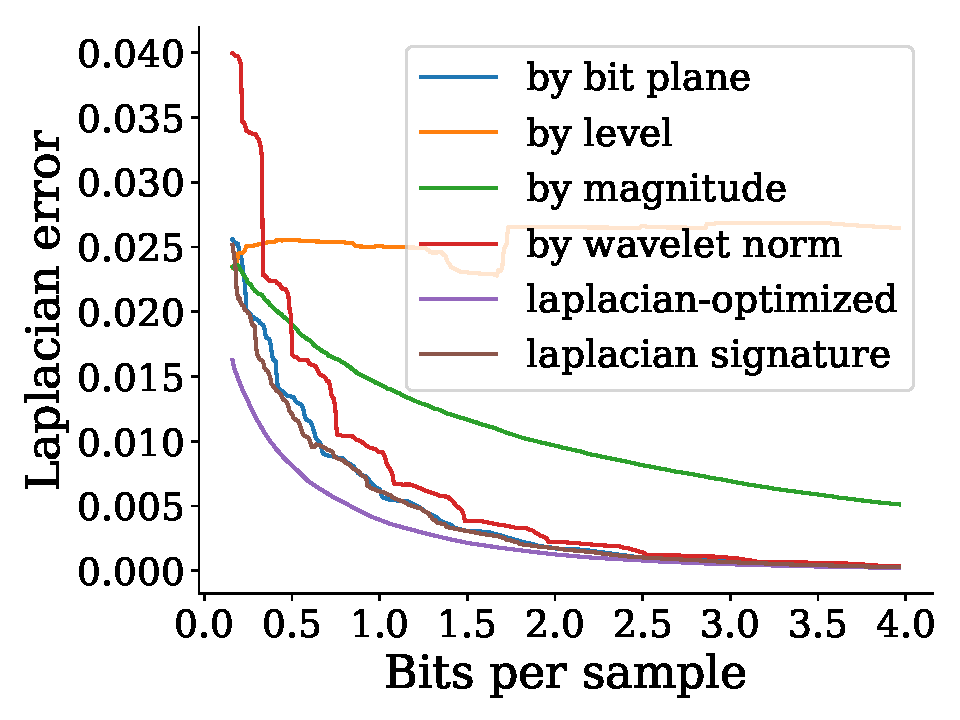
\includegraphics[width=0.24\linewidth]{laplacian/laplacian-optimized-diffusivity}}
\subcaptionbox{\emph{turbulence}}
{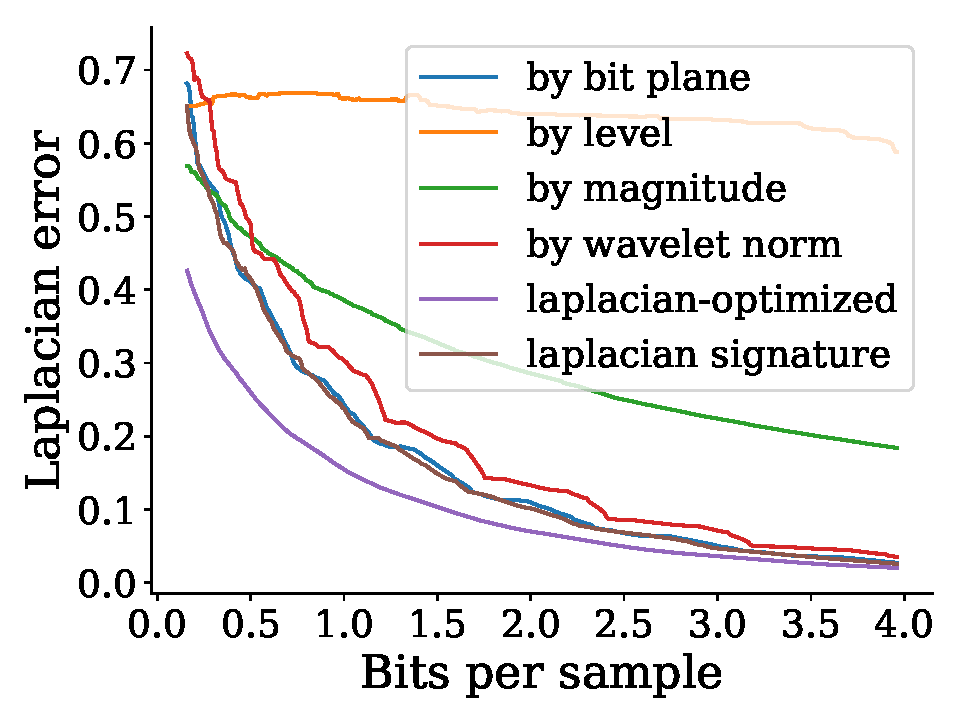
\includegraphics[width=0.24\linewidth]{laplacian/laplacian-optimized-turbulence}}
\subcaptionbox{\emph{pressure}}
{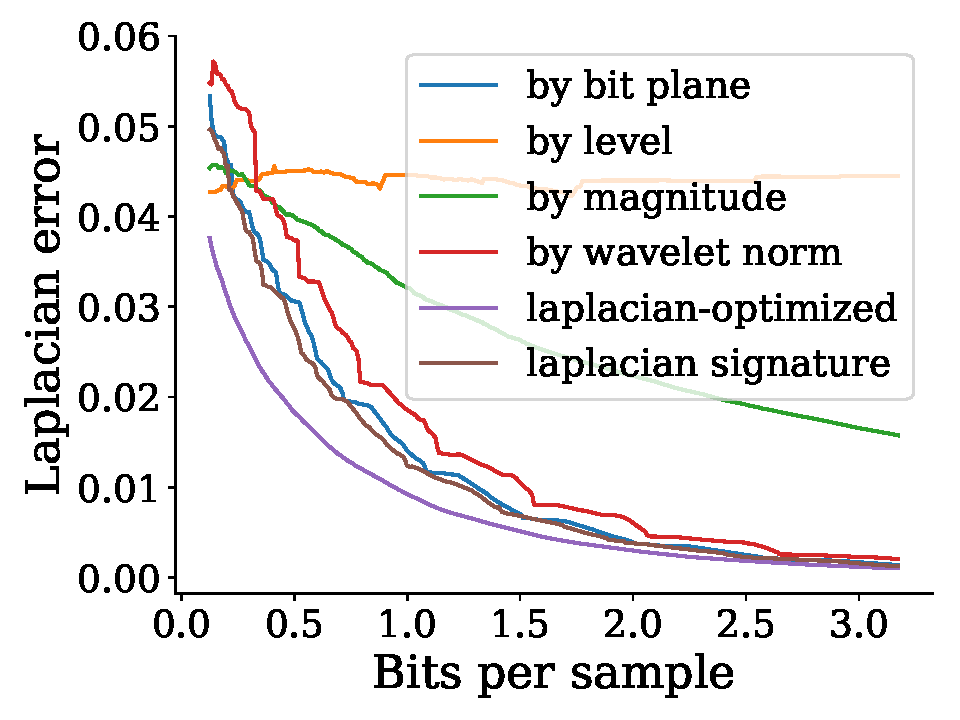
\includegraphics[width=0.24\linewidth]{laplacian/laplacian-optimized-pressure}}
\caption{Laplacian error comparison among streams. The plots are truncated to better highlight
differences without discarding important information. In all cases, in terms of error, $\slop <
\slsg < \sbit < \swav < \smag < \slvl$}.
\label{fig:laplacian-error-comparison}
\vspace{1em}
\end{figure*}

The Laplace operator is a second-order differential operator defined as the divergence of the
gradient field. The Laplacian of a 3D field is defined as $\Delta
f=\frac{{\partial}^2}{\partial{x^2}}f+\frac{{\partial}^2}{\partial{y^2}}f+\frac{{\partial}^2}{\partial{z^2}}f$.

Using a five-point finite difference, we approximate $\frac{{\partial}^2}{\partial{x^2}}f(x,y,z)
\approx
-\frac{1}{12}f(x-2,y,z)+\frac{4}{3}f(x-1,y,z)-\frac{5}{2}f(x,y,z)+\frac{4}{3}f(x+1,y,z)-\frac{1}{12}f(x+2,y,z)$.
We use the root-mean-square error to compare two Laplacian fields, i.e., $\err(\Delta
\tilde{f},\Delta f)=\text{RMSE}(\Delta \tilde{f},\Delta f)$. As usual, we use~\Cref{alg:greedy} to
compute a \emph{Laplacian-optimized} stream, \slop, which minimizes $\err$, and an \slsg stream from
its signature.~\Cref{fig:laplacian-error-comparison} plots the error curves for all relevant
streams. The plots here largely follow the ones in~\Cref{fig:gradient-error-comparison}, in terms of
relative performance among the streams, but with more discernible gaps between \sbit and \slsg.

\subsection{Histogram Computation}\label{sec:histogram}

A histogram succinctly summarizes the distribution of sample values, and thus is useful as a cursory
``look'' into the data and in guiding further analysis. For example, it can be used to guide the
selection of colors and opacities in a transfer function.

To decide on an error metric to compare histograms, we have experimented with several popular
metrics such as Kolmogorov-Smirnov~\cite{smirnov1948}, Kullback-Leibler~\cite{kullback1951}, and
Earth Mover's Distance~\cite{emd1998} among others~\cite{Hellinger1909,Bhattacharyya1943}. We choose
histogram intersection~\cite{histogram_intersection1991} as the metric of choice, because it is fast
to compute and is reasonably insensitive to changes in precision, as well as the number of bins. The
intersection distance between two histograms $H_1$ and $H_2$ is defined as
$\err(H_1,H_2)=1-\sum_{i}{\min{(H_1(i),H_2(i))}}$ (the sum is over all bins $i$). Every histogram is
normalized by dividing the value in each bin by the number of samples in the volume. We have decided
that the error metric should take into account both the histogram shapes and the range of values.
Therefore, we clamp the range of values in reconstructed functions to that of the original function,
so that corresponding histogram bins, i.e., $H_1(i)$ and $H_2(i)$, share the same range. However, in
situations where only the histogram shape but not the range of values is deemed important, no
clamping is needed.

As before, for each data set, we use~\Cref{alg:greedy} to compute an \shop stream, optimized for
histogram error, and then construct an \shsg from its signature. We plot the error curves for all
relevant streams using the Intersection error metric~(compare
\Cref{fig:histogram-stream-comparison}). We use 64 for the number of bins, but note that there exist
no meaningful differences across a wide range of number of bins (from 64 to 512) in our experiments.
In all cases, the group consisting of \sbit, \slvl, and \smag underperforms the other group by a
large margin.

Among the former group of streams, \slvl generally outperforms \sbit at low bit rates, although
there are several crossover points between the two curves~(visualization
in~\Cref{fig:histogram-explain}). When leading zero packets are present, \slvl outperforms \sbit,
because increasing resolution does not help produce an accurate histogram as much as increasing
precision. The histogram is oblivious to spatial locations of samples (which require resolution to
resolve), but is sensitive to sample values (which require precision). However, when leading zero
packets are removed with compression, \sbit benefits significantly more than \slvl does (for the
same reason explained in~\Cref{sec:rmse-optimized}), resulting in the observed crossovers. Finally,
\smag performs poorly, because it ignores regions of smooth variations, which nevertheless count
toward the distribution.

In the latter group, the performances of \swav and \shsg (and even \shop) differ by a negligible
amount. This observation is confirmed in~\Cref{fig:histograms-boiler}, where we plot various
histograms, reconstructed at 0.13 bps, for the \emph{boiler} data set. The histograms produced by
\swav and \shsg have approximately the same shape, and are the closest to the reference histogram.
The next best histogram is produced by \slvl, followed by the one produced by \sbit, and finally
\smag. These results suggest that histogram computation, while being in favor of precision, benefits
significantly from a bit ordering that combines both resolution and precision, not one that adheres
to either exclusively.

\begin{figure*}[t]
	\centering
	\subcaptionbox{\emph{boiler}}
	{\includegraphics[width=0.24\linewidth]{histogram/histogram-optimized-boiler}}
	\subcaptionbox{\emph{diffusivity}}
	{\includegraphics[width=0.24\linewidth]{histogram/histogram-optimized-diffusivity}}
	\subcaptionbox{\emph{kingsnake}}
	{\includegraphics[width=0.24\linewidth]{histogram/histogram-optimized-kingsnake}}
	\subcaptionbox{\emph{foam}}
	{\includegraphics[width=0.24\linewidth]{histogram/histogram-optimized-foam}}
	\caption{Comparison of histogram errors among streams. Plots are truncated to highlight
	differences without hiding important trends. In general, in terms of error, $\shop \approx \shsg
	\approx \swav < \slvl, \sbit, \smag$. The erratic behavior at the beginning for \emph{kingsnake}
	is likely due to the data being too noisy. The especially poor performances of \sbit for
	\emph{boiler} and \emph{foam} are due to the ``shifting'' effect explained in~\Cref{sec:gradient}.
	Crossover points between \sbit and \slvl are explained in~\Cref{fig:histogram-explain}}.
	\label{fig:histogram-stream-comparison}
\vspace{1em}

	\centering
	\subcaptionbox{\emph{by level} (\slvl)}{
	{\includegraphics[width=0.155\linewidth]{histogram/histogram-boiler-level.png}}}
	\subcaptionbox{\emph{by bit plane} (\sbit)}{
	{\includegraphics[width=0.155\linewidth]{histogram/histogram-boiler-bit-plane.png}}}
	\subcaptionbox{\emph{by magnitude} (\smag)}{
	{\includegraphics[width=0.155\linewidth]{histogram/histogram-boiler-magnitude.png}}}
	\subcaptionbox{\emph{by wavelet norm} (\swav)}{
	{\includegraphics[width=0.155\linewidth]{histogram/histogram-boiler-wavelet-norm.png}}}
	\subcaptionbox{\emph{by signature} (\shsg)}{
	{\includegraphics[width=0.155\linewidth]{histogram/histogram-boiler-signature.png}}}
	\subcaptionbox{\emph{reference}}{
	{\includegraphics[width=0.155\linewidth]{histogram/histogram-boiler-groundtruth.png}}}
	\caption{Histograms of the \emph{boiler} data set, reconstructed at 0.13 bps. \slvl, \swav, and
	\shsg produce histograms that share a shape similar to the reference histogram, with most of the
	peaks and valleys preserved. In contrast, \sbit produces a spurious peak not found in the
	reference. Finally, \smag's histogram has a widely skewed distribution where too many values fall
	into the first bin.}
	\label{fig:histograms-boiler}
	\vspace{-1em}
\end{figure*}

\begin{figure*}[t]
\centering
\subcaptionbox{\em pressure, isovalue=0.2}
{\includegraphics[width=0.24\linewidth]{isocontour/isocontour-optimized-pressure}}
\subcaptionbox{\em kingsnake, isovalue=106}
{\includegraphics[width=0.24\linewidth]{isocontour/isocontour-optimized-kingsnake}}
\subcaptionbox{\em plasma, isovalue=2}
{\includegraphics[width=0.24\linewidth]{isocontour/isocontour-optimized-plasma}}
\subcaptionbox{\em turbulence, isovalue=2}
{\includegraphics[width=0.24\linewidth]{isocontour/isocontour-optimized-turbulence}}
\caption{Comparison of isosurface errors among streams. Plots are truncated to highlight differences
without hiding important trends. In all cases, \slvl performs significantly worse than the rest.
\swav outperforms \sbit for \emph{pressure} and \emph{kingsnake}, but not for \emph{plasma} and \emph{turbulence}.}\label{fig:isocontour-plots}
\vspace{1em}

\centering
\subcaptionbox{\emph{by level} ($s_{lvl}$)}
{\includegraphics[width=0.16\linewidth]{isocontour/isocontour-level}}
\subcaptionbox{\emph{by bit plane} ($s_{bit}$)}
{\includegraphics[width=0.16\linewidth]{isocontour/isocontour-bit-plane}}
\subcaptionbox{\emph{by wavelet norm} ($s_{wav}$)}
{\includegraphics[width=0.16\linewidth]{isocontour/isocontour-wavelet-norm}}
\subcaptionbox{\emph{by magnitude} ($s_{mag}$)}
{\includegraphics[width=0.16\linewidth]{isocontour/isocontour-magnitude}}
\subcaptionbox{\emph{by signature} ($s_{iso-sig}$)}
{\includegraphics[width=0.16\linewidth]{isocontour/isocontour-signature}}
\subcaptionbox{\emph{ground truth}}
{\includegraphics[width=0.16\linewidth]{isocontour/isocontour-groundtruth}}
\caption{Rendering of isosurfaces at isovalue of 0.2, at 0.7 bps, for the \emph{pressure} data set.
The surfaces are colored by the $x$-component of the normal vector at each point. \swav and
\sisg produce surfaces that are closest to the reference, followed by \sbit, \smag, and \slvl.}
\label{fig:isocontour-surfaces-pressure}
\end{figure*}

\begin{figure}[h]
	\centering
	\subcaptionbox{with leading zero packets}
	{\includegraphics[width=0.48\linewidth]{histogram/histogram-explain-boiler-wlz}}
	\subcaptionbox{without leading zero packets}
	{\includegraphics[width=0.48\linewidth]{histogram/histogram-explain-boiler}} \caption{Histogram
	error curves produced by \sbit and \slvl, for \emph{boiler}, with and without leading zero bits.
	The vertical axis is in log scale. The error for \sbit reduces in a stair-step fashion, whhere
	each step corresponds to a new bit plane streamed. \sbit benefits significantly more from the
	removal of leading zero bits (the blue curve shifts more to the left).}
	\label{fig:histogram-explain}
	\vspace{-1em}
\end{figure}

\subsection{Isosurface extraction\pavol{update plot text to isosurface}}
\label{sec:isocontour}
Another common visualization task is display of boundaries, usually done using isosurfaces. For example,
isosurface of OH concentration can separate burning and extinguished regions in a combustion simulation or
organs can be extracted from medical imaging by threshold on a CT scalars. Moreover, topological methods such as Reeb Graph is
defined by contracting isosurfaces to a point and building the structure from equivalence classes of isosurfaces.
Extraction of isosurfaces is therefore an essential task in any
visualization and analysis system. We thus study the characteristics of bit streams that
minimize errors in the reconstructed isosurfaces and compare those streams quantitatively and qualitatively.

\pavol{potentially weak point as we do not use any standard error metric here; is the relative surface area fudge
necessary for higher resolution datasets?}
As before, we begin by defining an error metric to compare isosurfaces. Commonly used metric is a Hausdorff
distance that measures the shortest path from a point on one surface to the other, and then taking maximum
of all those paths. Unfortunately, the distance is not very robust and can vary drastically with minor changes
in the surfaces. For example, a single perturbation in one of the two surfaces
can result in a large distance even when the surfaces are close to identical. Therefore, we use a number of
misclassified voxels as our distance which can be computed by counting all voxels that are either in surface $S_1$
and not surface $S_2$ or the other way. \pavol{not sure if following is needed}We have found that if the error caused by
switching off a chunk is too small (in orders of sub-pixel/sub-voxel), then the importance of the
chunk cannot be properly measured. We therefore amend the error metric by adding to it the relative
difference in area between two isosurfaces. This relative difference is, most of the time, a number
between $0$ and $1$, computed by the formula $|A(S_1)-A(S_2)|/A(S_1)$, where $A(S)$ is the area of
an isosurface $S$. The idea is that when the number number of misclassified voxels is less than $1$, the
error -- which is at the sub-voxel level -- is captured by the relative difference in contour length
instead.

With an error metric defined, we can compute an \emph{isosurface-optimized} stream for each data set in addition
to the other streams that are data independent (\Cref{fig:isocontour-plots}). The hypothesis is resolving an
isosurface is primarily affected by the domain resolution.
Both resolution and precision streams are bounded by Nquist limit, a fine isosurface detail may fail
to be resolved either due low resolution or precision. As expected, the {\em isosurface-optimize} stream performs
the best as it has the most freedom when reordering chunks. We observed close to no difference between {\em by bit
plane}, {\em by wavelet norm}, and {\em isosurface signature} streams. This result is primarily caused by the need for
resolution when extracting isosurfaces. For example, {\em by bit plane} stream will always load full resolution data and
vary only precision.

\begin{figure}
	\centering
	\subcaptionbox{pressure}
	{\includegraphics[width=0.48\linewidth]{isocontour/isocontour-optimized-pressure}}
	\subcaptionbox{turbulence}
	{\includegraphics[width=0.48\linewidth]{isocontour/isocontour-optimized-turbulence}}
	\subcaptionbox{plasma}
	{\includegraphics[width=0.48\linewidth]{isocontour/isocontour-optimized-plasma}}
	\subcaptionbox{diffusivity}
	{\includegraphics[width=0.48\linewidth]{isocontour/isocontour-optimized-diffusivity}}
	\caption{Isosurface errors for data-independent, \emph{isosurface-optimized}, and
                 {\em isosurface signature} streams. The bit rates are capped to highlight differences
                 among streams. The {\em by level} and {\em by magnitude} streams performs worst and the other remaining
                 streams have similar performance.}
	\label{fig:isocontour-plots}
\end{figure}

Qualitatively, we studied isosurfaces at specific bit rates for all streams. We were especially interested
at bit rates where the error is not exponentially decaying - the low bit rate isosurfaces do not resemble
the reference full data set isosurfaces. For example, at bit rate 0.4 the error curves are mostly flat and the gaps between
them result in isosurfaces with visible differences (\Cref{fig:isocontour-surfaces})).

\begin{figure}[h]
	\centering
	\subcaptionbox{\emph{by level}}
	{\includegraphics[width=0.31\linewidth]{isocontour/isocontour-pressure-level}}
	\subcaptionbox{\emph{by bit plane}}
	{\includegraphics[width=0.31\linewidth]{isocontour/isocontour-pressure-bit-plane}}
	\subcaptionbox{\emph{by wavelet norm}}
	{\includegraphics[width=0.31\linewidth]{isocontour/isocontour-pressure-wavelet-norm}}
	\subcaptionbox{\emph{by magnitude}}
	{\includegraphics[width=0.31\linewidth]{isocontour/isocontour-pressure-magnitude}}
	\subcaptionbox{\emph{groundtruth}}
	{\includegraphics[width=0.31\linewidth]{isocontour/isocontour-pressure-groundtruth}}
	\caption{Miranda pressure field isosurfaces at bitrate of 0.4 bps.\pavol{what isovalue?} Both {\em by level}
        and {\em by magnitude} stream exhibit severe blocking artifacts compared to the groundtruth. The other streams
        still show smear artifacts, but the overall structure of the isosurfaces is more round and closer to the
        reference.}
	\label{fig:isocontour-surfaces}
\end{figure}

\begin{figure}[h]
	\centering
	\subcaptionbox{\emph{reference}}
	{\includegraphics[width=0.31\linewidth]{isocontour/isocontour2-groundtruth}}
	\subcaptionbox{\emph{by bit plane}}
	{\includegraphics[width=0.31\linewidth]{isocontour/isocontour2-bit-plane}}
	\subcaptionbox{\emph{by wavelet norm}}
	{\includegraphics[width=0.31\linewidth]{isocontour/isocontour2-wavelet-norm}}
	\caption{Miranda pressure field isosurfaces at bitrate of 0.4 bps.\pavol{what isovalue?} Both {\em by level}
        and {\em by magnitude} stream exhibit severe blocking artifacts compared to the groundtruth. The other streams
        still show smear artifacts, but the overall structure of the isosurfaces is more round and closer to the
        reference.}
	\label{fig:isocontour-surfaces}
\end{figure}
%Figure 5: We show that the hybrid and isocontour can diverge somewhat for low-gradient contour.
%Valerio suggested here we coudl also build a "ramp" dataset at different angles and see if the two
%diverges more as the ramp become flatter.

%We argue that if the gradient is low, some noise bits at the end will make an impact, the isocontour
%is very sensitive to noise, and is in general not interesting or meaninfgul to extract.


In this section, we looked at isosurface results for all six streams. The {\em by level} and {\em by magnitude} streams
show blocking artifacts compared to the less severe smearing of {\em by wavelet norm} and {\em by precisio} streams. Therefore,
it seems that one of those latter streams combined with a spatial adaptivity would perform well when isosurface
extraction is desired.

\section{Conclusion}

We presented a study of tradeoff between resolution and precision for commonly used derived
scientific quantities such as RMSE, gradient, Laplacian, histogram, and isosurface.
During this study, we covered the gamut of scientific data sets, ranging from simulations
with smooth features or fine scale detail to image data with noisy parts\pavol{do we have plot of image data?}.
We showed that one stream type does not fit all analysis tasks, but some streams perform well
in most of them and may be useful in a new file format design.

We started with an evaluation of contemporary techniques for reducing resolution or precision.
The experiments showed that streaming only in resolution or precision is suboptimal for all
tested queries. We thus developed a tractable greedy algorithm for computing adaptive stream order
based on the particular task. The produced stream significantly\pavol{it would be good to quantify what
significantly means, 2x?} outperforms any stream that has
a fixed streaming order.

After establishing the greedy algorithm for computing a stream, we focused on each query and
investigated which queries have similar streams. This approach is important because if two streams
are very similar, we can precompute the stream order and apply the same ordering to different
queries.

For example, we learned that the RMSE stream is akin to the gradient stream, and thus only one
needs to be computed. Moreover, since RMSE optimizes for the function, the stream alongside
a good gradient approaches the function itself. In contrast, the gradient ignores the constant offest
of all samples, resulting in an inferior RMSE.


These results should be considered when designing a file format for scientic data. As future work,
we plan to create new file format that will incorporate the stream-ordering techniques we presented.
Additionally, such file format needs to support compression and spatial adaptivity to handle large-scale
data and fast queries. We are investigating if signatures can be used to handle
the spatial adaptivity. For example, we could extend the signature matrix to the tensor, with
the spatial index being the third dimension.


%% if specified like this the section will be committed in review mode
% \acknowledgments{
% The authors wish to thank A, B, and C. This work was supported in part by
% a grant from XYZ (\# 12345-67890).}

\clearpage
\clearpage

%\bibliographystyle{abbrv}
\bibliographystyle{abbrv-doi}
%\bibliographystyle{abbrv-doi-narrow}
%\bibliographystyle{abbrv-doi-hyperref}
%\bibliographystyle{abbrv-doi-hyperref-narrow}

\bibliography{egbibsample}
\end{document}

